% +------------------------------------------------------------------------+
% | CBP Reference Manual:  main.tex
% +------------------------------------------------------------------------+
% | Automatically generated driver file for the reference manual chapter
% | of this package. Do not edit manually, you may loose your changes.
% +------------------------------------------------------------------------+
\def\ccTagRmTrailingConst{\ccFalse}

% +------------------------------------------------------------------------+
% | Reference manual page: Convex_hull_d_ref/intro.tex
% +------------------------------------------------------------------------+

%\clearpage
%\section{Reference Pages for dD Convex Hulls and Delaunay Triangulations}
\ccRefChapter{dD Convex Hulls and Delaunay Triangulations\label{chap:convex_hull_d_ref}}
\ccChapterAuthor{Susan Hert \and Michael Seel}

A subset $S \subseteq \R^3$ is convex if for any two points $p$ and $q$
in the set the line segment with endpoints $p$ and $q$ is contained
in $S$. The convex hull\ccIndexMainItemDef{convex hull} of a set $S$ is 
the smallest convex set containing
$S$. The convex hull of a set of points $P$ is a convex 
polytope with vertices in $P$.  A point in $P$ is an extreme point 
(with respect to $P$)\ccIndexMainItemDef{extreme point} if it is a vertex 
of the convex hull of $P$.

\cgal\ provides functions for computing convex hulls in two, three 
and arbitrary dimensions as well as functions for testing if a given set of 
points in is strongly convex or not.  This chapter describes the class
available for arbitrary dimensions and its companion class for 
computing the nearest and furthest side Delaunay triangulation. 

\section{Classified Reference Pages}

\ccHeading{Concepts}

\ccRefConceptPage{ConvexHullTraits_d} \\
\ccRefConceptPage{DelaunayLiftedTraits_d} \\
\ccRefConceptPage{DelaunayTraits_d} \\

\ccHeading{Classes}

\ccRefIdfierPage{CGAL::Convex_hull_d_traits_3<R>} \\
\ccRefIdfierPage{CGAL::Convex_hull_d<R>}  \\
\ccRefIdfierPage{CGAL::Delaunay_d< R, Lifted_R >} 

\clearpage




% First: concepts
% \input{Linear_cell_complex_ref/LinearCellComplex.tex}

% +------------------------------------------------------------------------+
% | Reference manual page: LinearCellComplexTraits.tex
% +------------------------------------------------------------------------+
% | 04.02.2010   Guillaume Damiand
% | Package: Linear_cell_complex
% +------------------------------------------------------------------------+
\ccRefPageBegin
%%RefPage: end of header, begin of main body
% +------------------------------------------------------------------------+

\begin{ccRefConcept}{LinearCellComplexTraits}

Required types and functors for the \ccRefName\ concept. This
geometric traits concept is used in the \ccc{Linear_cell_complex}
class.  

% \ccRefines
% A model of the concept \ccc{Kernel} if \ccc{Ambiant_dimension==2} or 
% \ccc{Ambiant_dimension==3}; a model of the concept \ccc{Kernel_d} otherwise.

% \ccc{CopyConstructable}, \ccc{Assignable}.

\ccConstants
\ccVariable{static unsigned int ambient_dimension;}
{The ambient dimension, must be \mygt{}1.}

\ccTypes

% \ccNestedType{Kernel}{kernel type.}

\ccNestedType{FT}{a number type that is a model of FieldNumberType.}
\ccGlue
\ccNestedType{Point}{point type.}
\ccGlue
\ccNestedType{Vector}{vector type.}
% \ccGlue
% \ccNestedType{Iso_cuboid}{iso cuboid type.}

\ccHeading{Constructions}

\ccNestedType{Construct_translated_point}
{Functor that provides \ccc{Point operator() (const Point& p, const Vector& v)}, 
 which constructs the translation of point \ccc{p} by vector \ccc{v}, and
\ccc{Point operator() (const CGAL::Origin&, const Vector& v)}, 
 which constructs the translation of a point at the origin by vector \ccc{v}
(used in \ccc{Linear_cell_complex::barycenter}).}
\ccGlue
\ccNestedType{Construct_vector}
{Functor that provides \ccc{Vector operator() (const Point& p1, const Point& p2)} 
 which constructs a vector as the difference of points \ccc{p2-p1}, and
 \ccc{Vector operator() (const CGAL::Origin&, const Point& p)} 
 which constructs a vector as the difference of point \ccc{p} and a point at the origin
(used in \ccc{Linear_cell_complex::barycenter} and \ccc{CGAL::import_from_plane_graph}).}
\ccGlue
\ccNestedType{Construct_sum_of_vectors}
{Functor that provides \ccc{Vector operator() (const Vector& v1, const Vector& v2)} 
 which constructs a vector as the sum of vectors \ccc{v1+v2}
(used in \ccc{Linear_cell_complex::barycenter}, \ccc{CGAL::compute_normal_of_cell_0} 
 and \ccc{CGAL::compute_normal_of_cell_2}).}
\ccGlue
\ccNestedType{Construct_scaled_vector}
{Functor that provides \ccc{Vector operator() (const Vector& v, FT scale)}
  which constructs a vector equal to vector \ccc{v} scaled by \ccc{scale} factor
(used in \ccc{Linear_cell_complex::barycenter} , \ccc{CGAL::compute_normal_of_cell_0}
 and \ccc{CGAL::compute_normal_of_cell_2}).}
\ccGlue
\ccNestedType{Construct_midpoint}
{Functor that provides \ccc{Point operator() (const Point& p1, const Point& p2)}
  which constructs the midpoint of points \ccc{p1} and \ccc{p2}
(used in \ccc{Linear_cell_complex::barycenter}).}

\textbf{If \ccc{ambient_dimension==2}}\\
\ccNestedType{Direction_2}{a model of \ccc{Direction_2}.}
\ccGlue
\ccNestedType{Construct_direction_2}
{a model of \ccc{ConstructDirection_2} (used in \ccc{CGAL::import_from_plane_graph}).}

\textbf{If \ccc{ambient_dimension==3}}\\
\ccNestedType{Construct_normal_3}
{a model of \ccc{ConstructNormal_3} (used in \ccc{CGAL::compute_normal_of_cell_2}).}
\ccNestedType{Collinear_3}
{a model of \ccc{Collinear_3} (used in \ccc{CGAL::compute_normal_of_cell_2}).}

\ccHasModels

\ccRefIdfierPage{CGAL::Linear_cell_complex_traits<d,K>}.

\ccSeeAlso

\ccRefIdfierPage{CGAL::Linear_cell_complex<d,d2,Traits_,Items_,Alloc_>}\\
%\ccRefConceptPage{LinearCellComplex}\\
\ccRefConceptPage{LinearCellComplexItems}\\

\end{ccRefConcept}
% +------------------------------------------------------------------------+
%%RefPage: end of main body, begin of footer
\ccRefPageEnd
% EOF
% +------------------------------------------------------------------------+


% +------------------------------------------------------------------------+
% | Reference manual page: LinearCellComplexItems.tex
% +------------------------------------------------------------------------+
% | 04.02.2010   Guillaume Damiand
% | Package: Combinatorial_map
% +------------------------------------------------------------------------+
\ccRefPageBegin
%%RefPage: end of header, begin of main body
% +------------------------------------------------------------------------+

\begin{ccRefConcept}{LinearCellComplexItems}

\ccDefinition The concept \ccRefName\ refines the concept of
\ccc{CombinatorialMapItems} by adding the requirement that
0-attributes are enabled, and associated with attributes which are a
model of the \ccc{CellAttributeWithPoint} concept.

% In addition to the requirements of \ccc{CombinatorialMapItems},
% the item class must also define the \ccc{Traits} type for the
% geometrical traits used, a model of the \ccc{LinearCellComplexTraits}
% concept.

% , and
% must define a \ccc{static const int ambient_dimension} for the
% dimension of the ambient space.

\ccRefines
\ccRefConceptPage{CombinatorialMapItems}

% +-----------------------------------+
\ccHeading{Requirements}

The first type in \ccc{Attributes} must be a model of the  
\ccc{CellAttributeWithPoint} concept.
% \item \ccc{dimension}$\leq$\ccc{ambient_dimension} (?).

% \ccTypes
% \ccNestedType{Traits}{a model of the \ccc{LinearCellComplexTraits} concept.}

% \ccConstants
% \ccVariable{static unsigned int ambient_dimension;}
% {The dimension of the ambient space.}

\ccHasModels
%\ccRefIdfierPage{CGAL::Linear_cell_complex_min_items<d,d2,Traits>}
\ccRefIdfierPage{CGAL::Linear_cell_complex_min_items<d>}

\ccSeeAlso
\ccRefIdfierPage{CGAL::Linear_cell_complex<d,d2,Traits_,Items_,Alloc_>}\\
\ccRefConceptPage{CellAttributeWithPoint}\\
%\ccRefConceptPage{LinearCellComplexTraits}\\
\ccRefIdfierPage{CGAL::Dart<d,CMap>}

\end{ccRefConcept}

% +------------------------------------------------------------------------+
%%RefPage: end of main body, begin of footer
\ccRefPageEnd
% EOF
% +------------------------------------------------------------------------+


% +------------------------------------------------------------------------+
% | Reference manual page: CombinatorialMapWithPoints.tex
% +------------------------------------------------------------------------+
% | 04.02.2010   Guillaume Damiand
% | Package: Combinatorial_map
% +------------------------------------------------------------------------+
\ccRefPageBegin
%%RefPage: end of header, begin of main body
% +------------------------------------------------------------------------+
\begin{ccRefConcept}{CellAttributeWithPoint}

\ccDefinition
  
The concept \ccRefName\ is a refinement of the \ccc{CellAttribute}
concept, to represent a cell attribute containing a point.
% For that, it refines a point concept wich can be either 
% \ccc{Kernel::Point_2} or \ccc{Kernel::Point_3} or \ccc{Kernel::Point_d} concept.

\ccRefines
\ccRefConceptPage{CellAttribute}  % \\

% If \ccc{ambient_dimension==2} \ccRefConceptPage{Kernel::Point_2}\\
% If \ccc{ambient_dimension==3} \ccRefConceptPage{Kernel::Point_3}\\
% Otherwise \ccRefConceptPage{Kernel::Point_d}


\ccTypes
%\ccParameters
% \ccc{Refs} must be a model of the \ccc{CombinatorialMap} concept.
% \ccc{T} must be \ccc{Tag_true} to enable the storage of a
% \ccc{Dart_handle} within the class (to be set to a dart which is part of the cell),
% and \ccc{Tag_false} otherwise.
% \ccNestedType{Traits}{The traits class, a model of the \ccc{LinearCellComplexTraits} concept.}
% \ccGlue
\ccNestedType{Point}{Type of the used point.} % Equals to \ccc{Traits::Point}.}

% A model of
%  \ccc{Kernel::Point_2} if \ccc{ambient_dimension==2},
%  a model of \ccc{Kernel::Point_3} if \ccc{ambient_dimension==3},
%  or a model of \ccc{Kernel::Point_d} otherwise.}

% \ccc{FunctorOnMerge} functor used when two cell attributes are merged. Must contains a method \ccc{operator ()} taking two \ccc{CellAttribute} as parameters.
% \ccc{FunctorOnSplit} functor used when one cell attribute was split in two. Must contains a method \ccc{operator ()} taking two \ccc{CellAttribute} as parameters.

% This concept does not have any restriction on the number
% of additional template parameters.

% \ccTypes

% \ccNestedType{Supports_cell_dart}
%     {equal to T (\ccc{Tag_true} or \ccc{Tag_false}).}
% +-----------------------------------+
% \ccConstants
% \ccVariable{static unsigned int ambient_dimension;}{The dimension of the ambient space.}

% +-----------------------------------+
\ccCreation
\ccCreationVariable{cawp}

\ccConstructor{CellAttributeWithPoint();}{Default constructor.}

\ccConstructor{CellAttributeWithPoint(const Point&apoint);}
   {Constructor initializing the point of \ccc{cawp} by the 
    copy contructor \ccc{Point(apoint)}.}

\ccConstructor{CellAttributeWithPoint(const Point&apoint, const Info& info);}
   {Constructor initializing the point of \ccc{cawp} by the 
    copy contructor \ccc{Point(apoint)} and initializing the
    information of \ccc{cawp} by the 
    copy contructor \ccc{Info(info)}.
    Defined only if \ccc{Info} is different from \ccc{void}.}

% +-----------------------------------+
\ccHeading{Access Member Functions}

\ccMethod{Point& point();} 
     {Returns the point of \ccc{cawp}.}

\ccMethod{const Point& point() const;} 
     {Returns the point of \ccc{cawp}, when \ccc{cawp} is const.}

\ccHasModels
\ccRefIdfierPage{CGAL::Cell_attribute_with_point<LCC,Info_,Tag,OnMerge,OnSplit>}
%\ccRefIdfierPage{CGAL::Cell_attribute_with_point_and_info}\\

\ccSeeAlso
%\ccRefConceptPage{LinearCellComplex}\\
\ccRefConceptPage{LinearCellComplexItems}
%\ccRefConceptPage{LinearCellComplexTraits}\\

\end{ccRefConcept}
% +------------------------------------------------------------------------+
%%RefPage: end of main body, begin of footer
\ccRefPageEnd
% EOF
% +------------------------------------------------------------------------+


%\input{Linear_cell_complex_ref/LinearCellComplexTraitsVector.tex}

% Second: classes
% Here we usae providecommand in case of Combinatorial_map.tex was used before
% this file.
\providecommand{\nulldart}{\ccc{null\_dart\_handle}}

\providecommand{\betats}{\ccTexHtml{$\beta$}{&beta;}}
\providecommand{\betazero}{\ccTexHtml{$\beta_0$}{&beta;<SUB>0</SUB>}}
\providecommand{\betaun}{\ccTexHtml{$\beta_1$}{&beta;<SUB>1</SUB>}}
\providecommand{\betadeux}{\ccTexHtml{$\beta_2$}{&beta;<SUB>2</SUB>}}
\providecommand{\betatrois}{\ccTexHtml{$\beta_3$}{&beta;<SUB>3</SUB>}}
\providecommand{\betaquatre}{\ccTexHtml{$\beta_4$}{&beta;<SUB>4</SUB>}}
\providecommand{\betai}{\ccTexHtml{$\beta_i$}{&beta;<SUB>i</SUB>}}
\providecommand{\betad}{\ccTexHtml{$\beta_d$}{&beta;<SUB>d</SUB>}}	
\providecommand{\betadprim}{\ccTexHtml{$\beta_{d'}$}{&beta;<SUB>d'</SUB>}}
\providecommand{\betaimun}{\ccTexHtml{$\beta_{i-1}$}{&beta;<SUB>i-1</SUB>}}
\providecommand{\betaipun}{\ccTexHtml{$\beta_{i+1}$}{&beta;<SUB>i+1</SUB>}}
\providecommand{\betaimdeux}{\ccTexHtml{$\beta_{i-2}$}{&beta;<SUB>i-2</SUB>}}
\providecommand{\betaipdeux}{\ccTexHtml{$\beta_{i+2}$}{&beta;<SUB>i+2</SUB>}}
\providecommand{\betaj}{\ccTexHtml{$\beta_j$}{&beta;<SUB>j</SUB>}}
\providecommand{\betajmun}{\ccTexHtml{$\beta_{j-1}$}{&beta;<SUB>j-1</SUB>}}
\providecommand{\betaiinv}{\ccTexHtml{$\beta_i^{-1}$}{&beta;<sub>i</sub><sup>-1</sup>}}
\providecommand{\betajinv}{\ccTexHtml{$\beta_j^{-1}$}{&beta;<sub>j</sub><sup>-1</sup>}}

\providecommand{\comp}{\ccTexHtml{$\circ$}{&deg;}}
\providecommand{\pinv}{\ccTexHtml{$p^{-1}$}{p<SUP>-1</SUP>}}
\providecommand{\myith}{\ccTexHtml{$i^{\mbox{th}}$}{i<SUP>th</SUP>}}

\providecommand{\myneq}{\ccTexHtml{$\neq$}{&ne;}}
\providecommand{\myleq}{\ccTexHtml{$\leq$}{&le;}}
\providecommand{\mylt}{\ccTexHtml{$<$}{&lt;}}
\providecommand{\mygt}{\ccTexHtml{$>$}{&gt;}}
\providecommand{\mygeq}{\ccTexHtml{$\geq$}{&ge;}}
\providecommand{\mysubseteq}{\ccTexHtml{$\subseteq$}{&sube;}}
\providecommand{\myforall}{\ccTexHtml{$\forall$}{&forall;}}
\providecommand{\myemptyset}{\ccTexHtml{$\emptyset$}{&empty;}}
\providecommand{\myRightarrow}{\ccTexHtml{$\Rightarrow$}{&rArr;}}
\providecommand{\myrightarrow}{\ccTexHtml{$\rightarrow$}{&rarr;}}
\providecommand{\myin}{\ccTexHtml{$\in$}{&isin;}}
\providecommand{\mynotin}{\ccTexHtml{$\notin$}{&notin;}}
\providecommand{\mycup}{\ccTexHtml{$\cup$}{&cup;}}
\providecommand{\myphi}{\ccTexHtml{$\phi$}{&phi;}}
\providecommand{\mysetminus}{\ccTexHtml{$\setminus$}{\ }}
\providecommand{\myldots}{\ccTexHtml{$\ldots$}{&hellip;}}
\providecommand{\mytimes}{\ccTexHtml{$\times$}{&times;}}

\providecommand{\cell}[1]{\emph{#1}-cell}
\providecommand{\cells}[1]{\emph{#1}-cells}
\providecommand{\orbit}[1]{\ccTexHtml{$\langle{}$}{&lang;}#1\ccTexHtml{$\rangle{}$}{&rang;}}




\section{Introduction}

A \emph{d}D linear cell complex allows to represent an orientable
subdivided \emph{d}D object having linear geometry: each vertex of the
subdivision is associated with a point. The geometry of each edge is a
segment whose end points are associated with the two vertices of the
edge, the geometry of each 2-cell is obtained from all the segments
associated to the edges describing the boundary of the 2-cell and so
on.

The combinatorial part of a linear cell complex is described by a
\emph{d}D combinatorial map (it is strongly recommended to first
read \ccRef[the combinatorial maps chapter]{ChapterCombinatorialMap}
for definitions).  To add
the linear geometrical embedding, a point (a model of
\ccc{CGAL::Point_2} or \ccc{CGAL::Point_3} or \ccc{CGAL::Point_d}) is
associated to each vertex of the combinatorial map.

%%%%%%%%%%%%%%%%%%%%%%%%%%%%%%%%%%%%%%%%%
\begin{figure}[ht]
  \begin{ccTexOnly}
    \begin{center}
      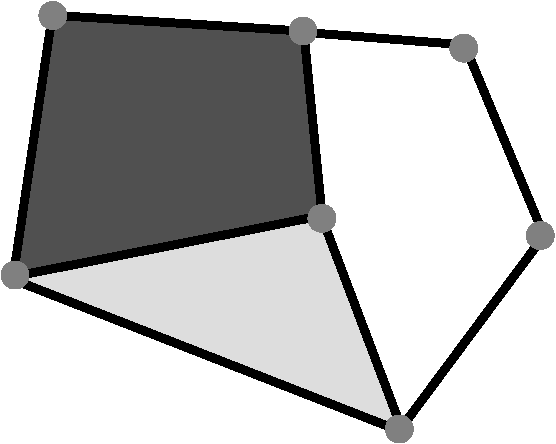
\includegraphics[width=.35\textwidth]
      {Linear_cell_complex/fig/pdf/object2d}
      \qquad
      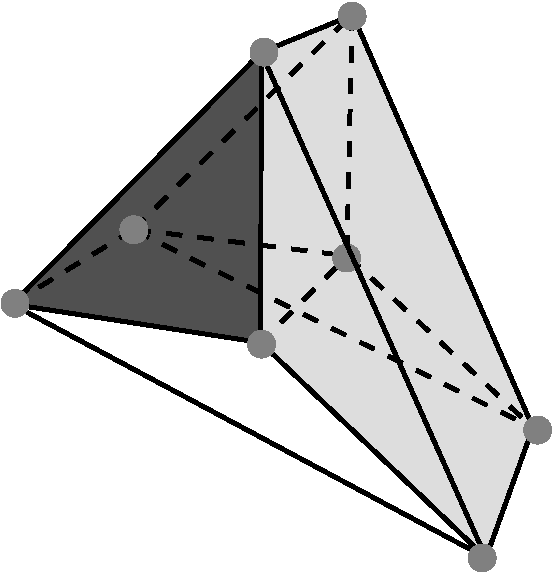
\includegraphics[width=.45\textwidth]
      {Linear_cell_complex/fig/pdf/intuitif-example-lcc-object}
    \end{center}
  \end{ccTexOnly}
  \begin{ccHtmlOnly}
    <CENTER>
    <A HREF="fig/png/object2d.png"><img src="fig/png/object2d.png" alt=""></A>
    <A HREF="fig/png/intuitif-example-lcc-object.png"><img src="fig/png/intuitif-example-lcc-object.png" alt=""></A>
    </CENTER>
    \end{ccHtmlOnly}
    \caption{Examples of objects with linear geometry. \textbf{Left}:~A
      2D object composed of three 2-cells, nine
      1-cells and seven points associated to the seven 0-cells .   
      \textbf{Right}:~A
      3D object composed of three 3-cells, twelve 2-cells, sixteen
      1-cells and eight points associated to the eight 0-cells.
      \label{fig-exemple-introductif}}
\end{figure}
%
If we reconsider the example introduced in the combinatorial map
package, recalled in Figure~\ref{fig-exemple-introductif} (Right), the
combinatorial part of the 3D object is described by a 3D combinatorial
map. As illustrated in Figure~\ref{fig-exemple-introductif-lcc}, the
geometrical part of the object is described by associating a point to
each vertex of the map.
%
\def\LargFig{.3\textwidth}
\begin{figure}[h]
  \begin{ccTexOnly}
    \begin{center}
      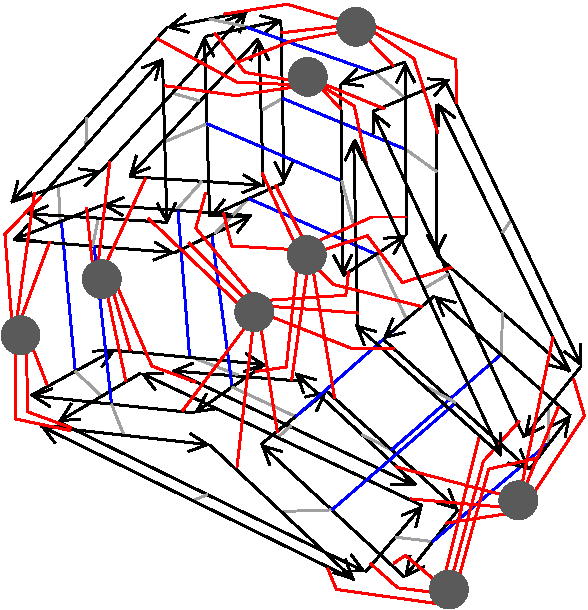
\includegraphics[width=\LargFig]{Linear_cell_complex/fig/pdf/intuitif-example-lcc}\qquad
      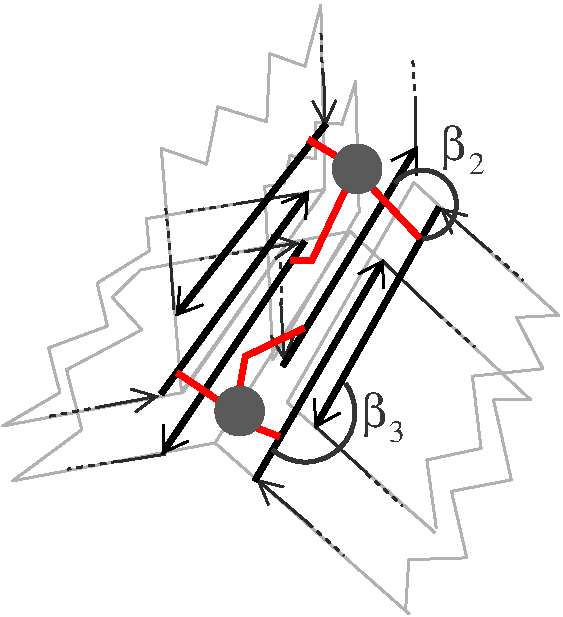
\includegraphics[width=\LargFig]{Linear_cell_complex/fig/pdf/intuitif-example-lcc-zoom}
      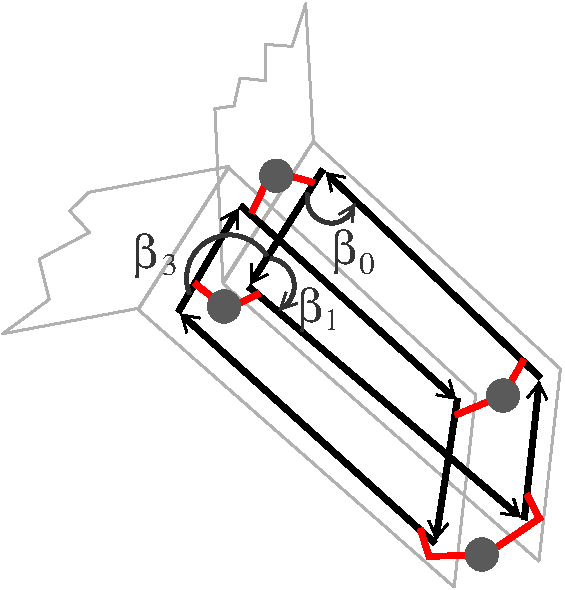
\includegraphics[width=\LargFig]{Linear_cell_complex/fig/pdf/intuitif-example-lcc-zoom2}
    \end{center}
  \end{ccTexOnly}
  \begin{ccHtmlOnly}
    <CENTER>
    <A HREF="fig/png/intuitif-example-lcc.png">
    <img src="fig/png/intuitif-example-lcc.png" alt=""></A>
    <A HREF="fig/png/intuitif-example-lcc-zoom.png">
        <img src="fig/png/intuitif-example-lcc-zoom.png" alt=""></A>
    <A HREF="fig/png/intuitif-example-lcc-zoom2.png">
        <img src="fig/png/intuitif-example-lcc-zoom2.png" alt=""></A>
    </CENTER>
    \end{ccHtmlOnly}
    \caption{Example of 3D linear cell complex describing the object
      given in Figure~\ref{fig-exemple-introductif} (Right).
      \textbf{Left}:~The 3D linear cell complex which contains 54 darts
      (18 for each 3-cell) where each vertex is associated with a
      point, here a \ccc{CGAL::Point_3}. Blue segments represent \betatrois{} relations.
      \textbf{Middle}:~Zoom around
      the central edge which details the six darts belonging to the
      edge and the associations between darts and points.
      \textbf{Right}:~Zoom around the facet between light gray and
      white 3-cells, which details the eight darts belonging to the
      facet and the associations between darts and
      points (given by red segments).\label{fig-exemple-introductif-lcc}}
\end{figure}

Note that the dimension of the combinatorial map \emph{d} is not
necessarily equal to the dimension of the ambient space
\emph{d2}. Indeed, we can use for example a 2D combinatorial map in a
2D ambient space to describe a planar graph
(\emph{d}=\emph{d2}=\emph{2}), or a 2D combinatorial map in a 3D
ambient space to describe a surface in 3D space (\emph{d}=2,
\emph{d2}=3) (case of the \ccc{Polyhedron_3} package), or a 3D
combinatorial map in a 3D ambient space (\emph{d}=\emph{d2}=3) and so
on.

\section{Software Design}

The diagram in Figure~\ref{fig-diagram_class_lcc} shows the main
classes of the package.  \ccc{CGAL::Linear_cell_complex} is the main
class (see Section~\ref{ssec-linear-cell-complex}), which inherits from
the \ccc{CGAL::Combinatorial_map} class.  Attributes can be associated
to some cells of the linear cell complex thanks to an items class (see
Section~\ref{ssec-lcc-item}), which defines the dart type and the
attributes types. These types may be different for different
dimensions of cells, and they may also be void.  In the class
\ccc{CGAL::Linear_cell_complex}, it is required that
specific attributes are associated to all vertices of the
combinatorial map. These attributes must contain a point (a model of
\ccc{CGAL::Point_2} or \ccc{CGAL::Point_3} or \ccc{CGAL::Point_d}),
and can be represented by instances of class
\ccc{CGAL::Cell_attribute_with_point} (see
Section~\ref{ssec-attribute-wp}).
%
\begin{figure}
  \begin{ccTexOnly}
    \begin{center}
      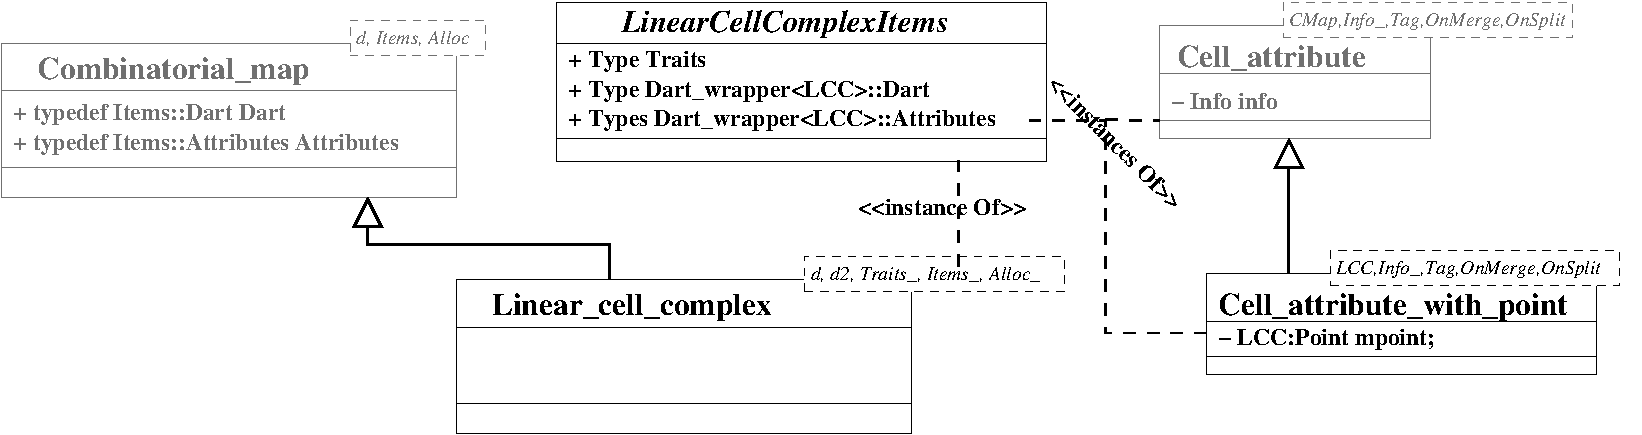
\includegraphics[width=.95\textwidth]
      {Linear_cell_complex/fig/pdf/Diagramme_class}
    \end{center}
  \end{ccTexOnly}
  \begin{ccHtmlOnly}
    <CENTER>
    <A HREF="fig/png/Diagramme_class.png">
        <img src="fig/png/Diagramme_class.png" alt=""></A>
    </CENTER>
    \end{ccHtmlOnly}
    \caption{UML diagram of the main classes of the package. Gray
      elements come from the 
      \ccRef[combinatorial map package]{ChapterCombinatorialMap}.}
    \label{fig-diagram_class_lcc}
\end{figure}

\subsection{Linear Cell Complex}\label{ssec-linear-cell-complex}

The \ccc{CGAL::Linear_cell_complex<d,d2,LCCTraits,CMItems,Alloc>} class
is a model of the \ccc{CombinatorialMap} concept. It guarantees that
each vertex of the combinatorial map is associated with an attribute
containing a point. This class can be used in geometric algorithms (it
plays the same role as \ccc{Polyhedron_3} for \ccc{HalfedgeDS}).

This class has five template parameters standing for the dimension of
the combinatorial map, the dimension of the ambient space, a traits
class (a model of the \ccc{LinearCellComplexTraits} concept, see
Section~\ref{ssec-lcc-traits}), an items class (a model of the
\ccc{LinearCellComplexItems} concept, see
Section~\ref{ssec-lcc-item}), and an allocator which must be a model
of the allocator concept of {\stl}.  Default classes are provided for
the traits, items, and for the allocator classes, and by default
\ccc{d2=d}.

A linear cell complex is valid, if it is a valid combinatorial map
where each dart is associated with an attribute containing a point
(i.e.  an instance of a model of the \ccc{CellAttributeWithPoint}
concept).  Note that there are no validity constraint on the geometry
(test on self intersection, planarity of 2-cells...).
We can see two examples of \ccc{CGAL::Linear_cell_complex} in
Figure~\ref{fig-combi_map_with_point}.

%%%%%%%%%%%%%%%%%%%%%%%%%%%%%%%%%%%%%%%%%%%%%%
\begin{figure}
\begin{ccTexOnly}
  \centerline{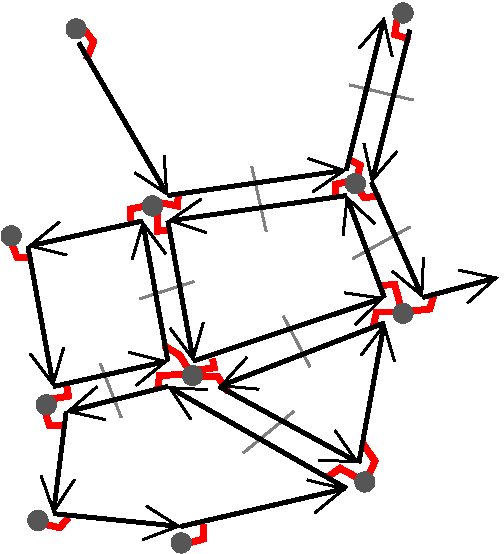
\includegraphics[width=.25\textwidth]
    {Linear_cell_complex/fig/pdf/plane-graph}
  \qquad
  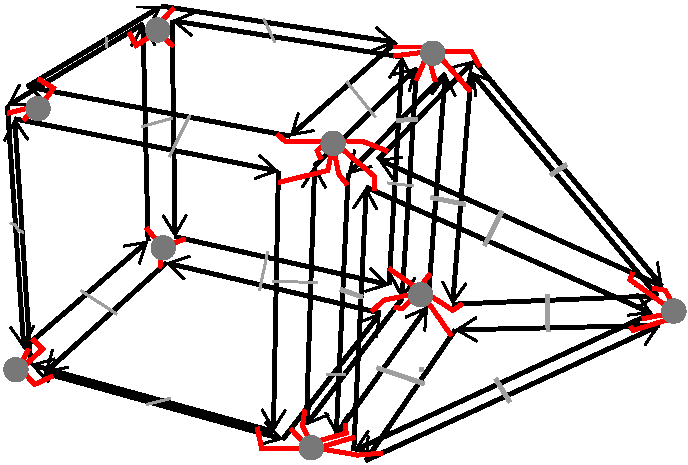
\includegraphics[width=.45\textwidth]
  {Linear_cell_complex/fig/pdf/basic-example3D}}
\end{ccTexOnly}
\begin{ccHtmlOnly}
  <CENTER>
  <A HREF="fig/png/plane-graph.png">
      <img src="fig/png/plane-graph.png" alt=""></A>
  <A HREF="fig/png/basic-example3D.png">
      <img src="fig/png/basic-example3D.png" alt=""></A>
  </CENTER>
\end{ccHtmlOnly}
\caption{Examples of \ccc{CGAL::Linear_cell_complex}. Gray disks show the
  attributes associated to vertices. Associations between darts and
  attributes are drawn by small lines between darts and disks.
  \textbf{Left:}~Example of \ccc{CGAL::Linear_cell_complex<2,2>}.
  \textbf{Right:}~Example of \ccc{CGAL::Linear_cell_complex<3,3>}.}
\label{fig-combi_map_with_point}
\end{figure}

\subsection{Cell Attributes}\label{ssec-attribute-wp}

The
\ccc{CGAL::Cell_attribute_with_point<LCC,Info_,Tag,OnMerge,OnSplit>}
class is a model of the \ccc{CellAttributeWithPoint} concept, which is
a refinement of the \ccc{CellAttribute} concept. It represents an
attribute associated with a cell, which can contain an information
(depending on whether \ccc{Info_==void} or not), but which always
contains a point, an instance of \ccc{LCC::Point}.

\subsection{Linear Cell Complex Traits}\label{ssec-lcc-traits}

The \ccc{LinearCellComplexTraits} geometric traits concept defines the
required types and functors used in the \ccc{Linear_cell_complex}
class. For example it defines \ccc{Point}, the type of points used,
and \ccc{Vector}, the corresponding vector type.  It also defines all
the required functors used for constructions and operations, as for
example \ccc{Construct_translated_point} or
\ccc{Construct_sum_of_vectors}.

The class \ccc{CGAL::Linear_cell_complex_traits<d,K>} is a model of
\ccc{LinearCellComplexTraits}. It defines the different types which
are obtained from \ccc{K} that, depending on \ccc{d}, is either a model of
the concept \ccc{Kernel} if \ccc{d==2} or \ccc{d==3}, a model of the
concept \ccc{Kernel_d} otherwise.


\subsection{Linear Cell Complex Items}\label{ssec-lcc-item}

The \ccc{LinearCellComplexItems} concept refines the
\ccc{CombinatorialMapItems} concept by adding the requirement that
0-attributes are enabled, and associated with a type of attribute
being a model of the \ccc{CellAttributeWithPoint} concept.  

The class \ccc{CGAL::Linear_cell_complex_min_items<d>} is a
model of \ccc{LinearCellComplexItems}. It uses \ccc{CGAL::Dart<d>},
and instances of \ccc{CGAL::Cell_attribute_with_point}
(which contain no information) associated to each vertex. All other
attributes are void.  

\section{Operations}

Several operations defined in the combinatorial maps package can be
used on a linear cell complex. This is the case for all the iteration
operations that do not modify the model (see example in 
Section~\ref{ssec-3D-lcc}). This is also the case for
all the operations that do not create new 0-cells: \ccc{sew},
\ccc{unsew}, \ccc{remove_cell}, \ccc{insert_cell_1_in_cell_2},
\ccc{insert_cell_2_in_cell_3}.  Indeed, all these operations update
non void attributes, and thus update vertex attributes of a linear
cell complex. Note that some existing 0-attributes can be duplicated
by the \ccc{unsew} method, but these 0-attributes are not new but
copies of existing old 0-attributes.

However, operations that create a new 0-cell can not be directly used
since the new 0-cell would not be associated with a vertex
attribute. Indeed, it is not possible for these operations to
automatically decide which point to create. These operations are:
\ccc{insert_cell_0_in_cell_1}, \ccc{insert_cell_0_in_cell_2}
\ccc{insert_dangling_cell_1_in_cell_2}, plus all the creation
operations. For these operations, new versions are proposed taking
some points as additional parameters.  Lastly, some new operations are
defined, which use the geometry (see Sections~\ref{ssec-constructions-op} and
\ref{ssec-modif-op}).

All the operations given in this section guarantee that given a valid
linear cell complex and a possible operation, the result is a valid
linear cell complex. As for a combinatorial map, it is also possible
to use low level operations but additional operations may be needed to
restore the validity conditions.

\subsection{Sewing and Unsewing \label{ssec-lcc-link-darts}}

As explained in the combinatorial map user manual,
Section~\ref{ssec-link-darts}, it is possible to glue two \emph{i}-cells
along an (\emph{i}-1)-cell by using the \ccc{sew<i>} method. Since
this method updates non void attributes, and since points are specific
attributes, they are automatically updated during the \ccc{sew<i>}
method. Thus the sewing of two \emph{i}-cells could deform the
geometry of the concerned objects.

For example, in Figure~\ref{fig-lcc-exemple-sew}, we want to 3-sew the
two initial 3-cells. \ccc{sew<3>(1,5)} links by \betatrois{} the pairs
of darts (1,5), (2,8), (3,7) and (4,6). The eight vertex attributes
around the facet between the two 3-cells before the sew are merged by
pair during the sew operation (and the \ccc{On_merge} functor is
called four times). Thus, after the sew, there are only four
0-attributes around the facet. By default, the attributes associated
with the first dart of the sew operation are kept (but this can be
modified by defining your own functor in the attribute class as
explained in the package combinatorial map, Section~\ref{ssec-link-darts}). 
Intuitively, the
geometry of the second 2-cell is deformed to fit to the first 2-cell.
%
\def\LargFig{.45\textwidth}
\begin{figure}
  \begin{ccTexOnly}
    \begin{center}
      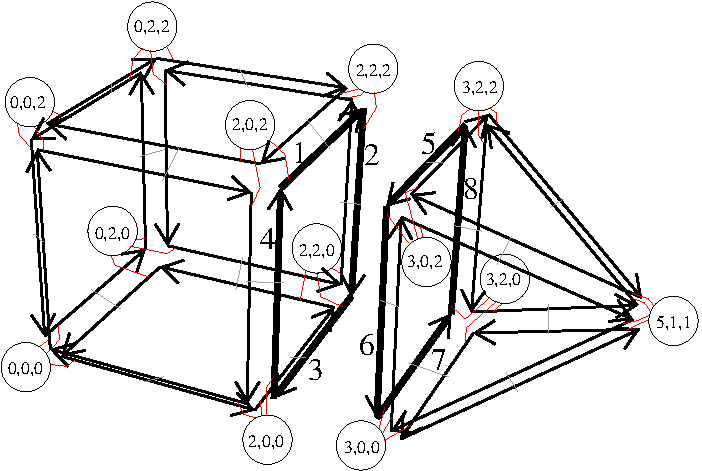
\includegraphics[width=\LargFig]{Linear_cell_complex/fig/pdf/exemple-carte-with_point_3d-sew}\qquad
      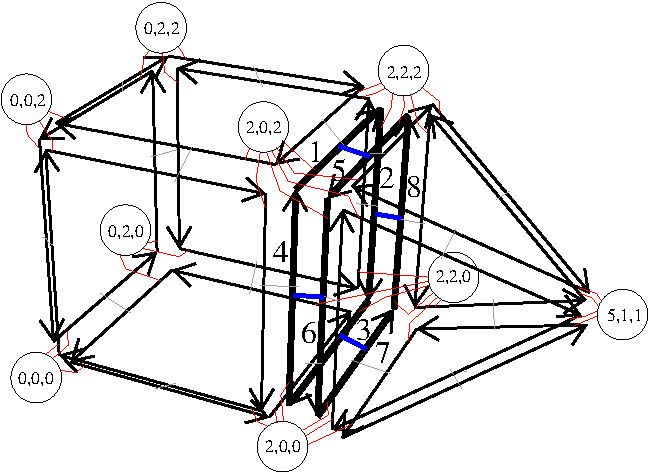
\includegraphics[width=\LargFig]{Linear_cell_complex/fig/pdf/exemple-carte-with_point_3d-sew2}
    \end{center}
  \end{ccTexOnly}
  \begin{ccHtmlOnly}
    <CENTER>
    <A HREF="fig/png/exemple-carte-with_point_3d-sew.png">
        <img src="fig/png/exemple-carte-with_point_3d-sew.png" alt=""></A>
    <A HREF="fig/png/exemple-carte-with_point_3d-sew2.png">
        <img src="fig/png/exemple-carte-with_point_3d-sew2.png" alt=""></A>
    </CENTER>
    \end{ccHtmlOnly}
    \caption{Example of 3-sew operation for linear cell complex.
      \textbf{Left}: A 3D linear cell complex containing two 3-cells
      that are not connected. Vertex attributes are drawn with circles
      containing point coordinates.  Associations between darts and
      attributes are drawn with small lines between darts and
      disks. \textbf{Right}: The 3D linear cell complex obtained as
      result of \ccc{sew<3>(1,5)} (or \ccc{sew<3>(2,8)}, or
      \ccc{sew<3>(3,7)}, or \ccc{sew<3>(4,6)}).  The eight
      0-attributes around the facet between the two 3-cells before the
      sew operation, are merged into four 0-attributes after. The
      geometry of the pyramid is deformed since its base is fitted on
      the 2-cell of the cube.}
    \label{fig-lcc-exemple-sew}
\end{figure} 

This is similar for the unsew operation, which removes \betai{} links
of all the darts in
\orbit{\betaun{},\myldots{},\betaimdeux{},\betaipdeux{},\myldots{},\betad{}}(\emph{d0}), 
and updates
non void attributes which are no more associated to a same cell due to
the unlinks.  If we take the linear cell complex given in
Figure~\ref{fig-lcc-exemple-sew} (Right), and we call
\ccc{unsew<3>(2)}, we obtain the linear cell complex in
Figure~\ref{fig-lcc-exemple-sew} (Left) except for the coordinates of
the new four vertices, which by default are copies of original
vertices (this behavior can be modified thanks to the functor
\ccc{On_split} in the attribute class).  The \ccc{unsew<3>} operation
has removed the four \betatrois{} links, and has duplicated the 0-attributes
since vertices are split in two after the unsew operation.

\subsection{Construction Operations}\label{ssec-constructions-op}

There are several member functions allowing to insert specific
configurations of darts into a linear cell complex. These functions
return a \ccc{Dart_handle} to the new object.  Note
that the dimension of the linear cell complex must be large enough:
darts must contain all the \betats{} used by the operation.  All these
methods add new darts in the current linear cell complex, existing
darts are not modified. These functions
are \ccc{make_segment}, \ccc{make_triangle}, 
\ccc{make_tetrahedron} and \ccc{make_hexahedron}. 

There are two functions allowing to build a linear cell complex
from two other \cgal\ data types:
\begin{itemize}
\item \ccc{import_from_triangulation_3(lcc,atr)}: adds in \ccc{lcc} all 
  the tetrahedra present in \ccc{atr}, a \ccc{CGAL::Triangulation_3};
\item \ccc{import_from_polyhedron_3(lcc,ap)}: adds in \ccc{lcc} all 
  the cells present in \ccc{ap}, a \ccc{CGAL::Polyhedron_3}.
\end{itemize}

Lastly, the function \ccc{import_from_plane_graph(lcc,ais)} adds in
\ccc{lcc} all the cells reconstructed from the planar graph read in
\ccc{ais}, a \ccc{std::istream} (see the reference manual for the file
format).

\subsection{Modification Operations}\label{ssec-modif-op}

Some methods are defined in \ccc{Linear_cell_complex} class
to modify a linear cell complex and update the vertex attributes.  In
the following, we denote by \ccc{dh0}, \ccc{dh1}, \ccc{dh2} the dart
handles for the darts \ccc{d0}, \ccc{d1}, \ccc{d2}, respectively. That
is \ccc{d0 == *dh0}.

%%%%%%%%%%%%%%%%%%%%%%%%%%%%%%%%%%%%%%%%%%%%%%%%%%%%%%%%%%%%%%%%%%%%%%%%%%%%%%
\begin{figure}[htb]
  \begin{ccTexOnly}
    \begin{center}
      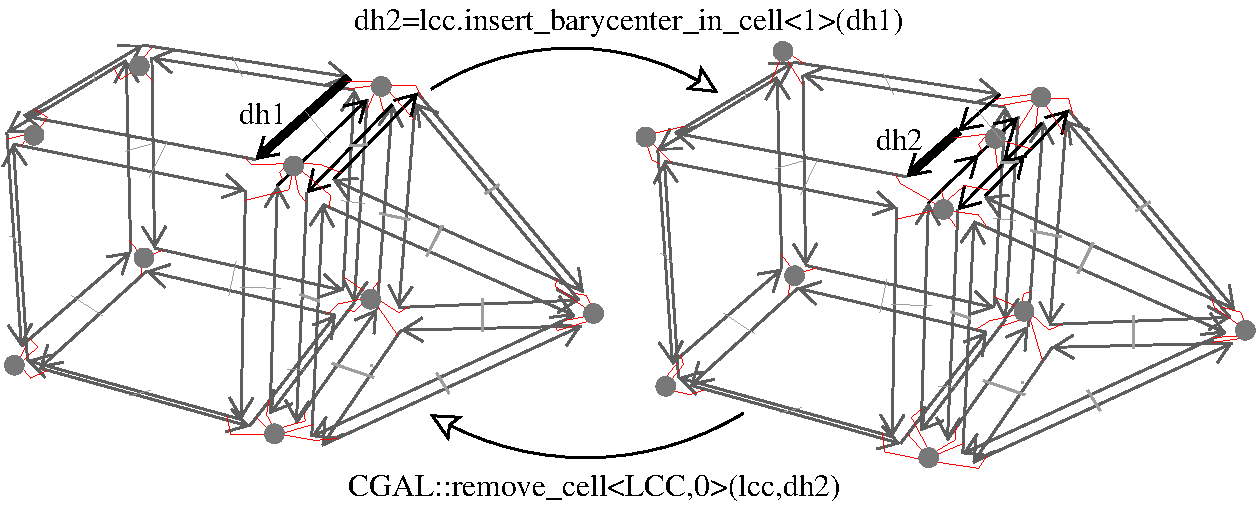
\includegraphics[width=.75\textwidth]{Linear_cell_complex/fig/pdf/insert-vertex}
    \end{center}
  \end{ccTexOnly}
  \begin{ccHtmlOnly}
    <CENTER> <A HREF="fig/png/insert-vertex.png"><img
    src="fig/png/insert-vertex.png" alt=""></A> </CENTER>
  \end{ccHtmlOnly}
  \caption{Example of \ccc{insert_barycenter_in_cell<1>} and
    \ccc{remove_cell<0>} operations. \textbf{Left}: Initial linear
    cell complex.  \textbf{Right}: After the insertion of a point in
    the barycenter of the 1-cell containing dart \emph{d1}.  Now if we
    remove the 0-cell containing dart \emph{d2}, we obtain a linear
    cell complex isomorphic to the initial one.}
  \label{fig-lcc-insert-vertex}
\end{figure}
%%%%%%%%%%%%%%%%%%%%%%%%%%%%%%%%%%%%%%%%%%%%%%%%%%%%%%%%%%%%%%%%%%%%%%%%%%%%%%

\ccc{lcc.insert_barycenter_in_cell<unsigned int i>(dh0)} adds the
barycenter of the \emph{i}-cell containing dart \ccc{d0}. This
operation is possible if \ccc{d0}\myin{}\ccc{lcc.darts()} (see examples
on Figure~\ref{fig-lcc-insert-vertex} and
Figure~\ref{fig-lcc-triangulate}).

\ccc{lcc.insert_point_in_cell<unsigned int i>(dh0,p)} is an operation
similar to the previous operation, the only difference being that the
coordinates of the new point are here given by \ccc{p} instead of being
computed as the barycenter of the \emph{i}-cell.  Currently, these two
operations are only defined for \ccc{i=1} to insert a point in an
edge, or \ccc{i=2} to insert a point in a facet.
\begin{figure}[htb]
  \begin{ccTexOnly}
    \centerline{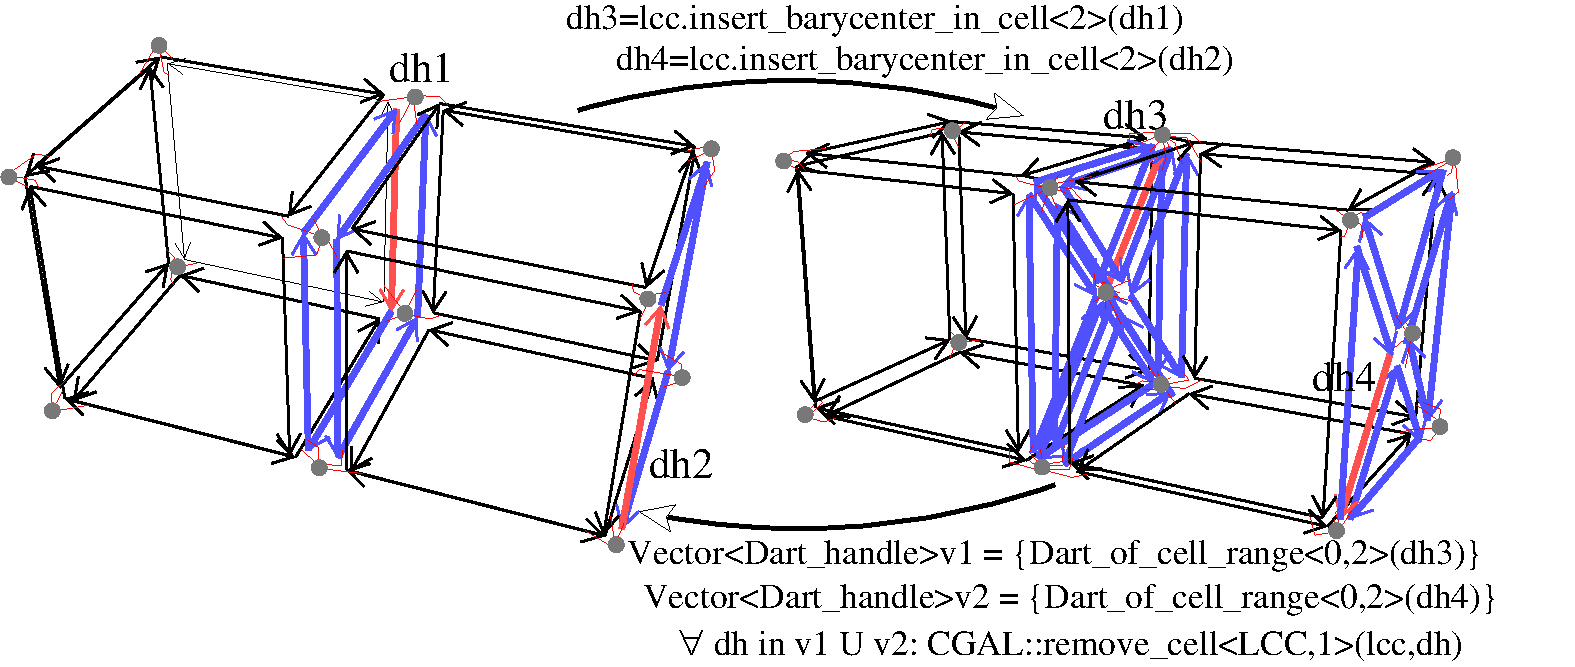
\includegraphics[width=.85\textwidth]
      {Linear_cell_complex/fig/pdf/triangulation}}
  \end{ccTexOnly}
  \begin{ccHtmlOnly}
    <CENTER> <A HREF="fig/png/triangulation.png"> <img
    src="fig/png/triangulation.png" alt=""></A> </CENTER>
  \end{ccHtmlOnly}
  \caption{Examples of \ccc{insert_barycenter_in_cell<2>} operation.}
  \label{fig-lcc-triangulate}
\end{figure}
%

\ccc{lcc.insert_dangling_cell_1_in_cell_2(dh0,p)} adds a 1-cell in
the 2-cell containing dart \ccc{d0}, the 1-cell being attached by only
one of its vertex to the 0-cell containing dart \ccc{d0}.  The second
vertex of the new edge is associated with a new 0-attribute containing
a copy of \ccc{p} as point. This operation is possible if
\ccc{d0}\myin{}\ccc{lcc.darts()} (see example on
Figure~\ref{fig-lcc-insert-dangling-edge}).
  \begin{figure}[htb]
    \begin{ccTexOnly}
      \begin{center}
        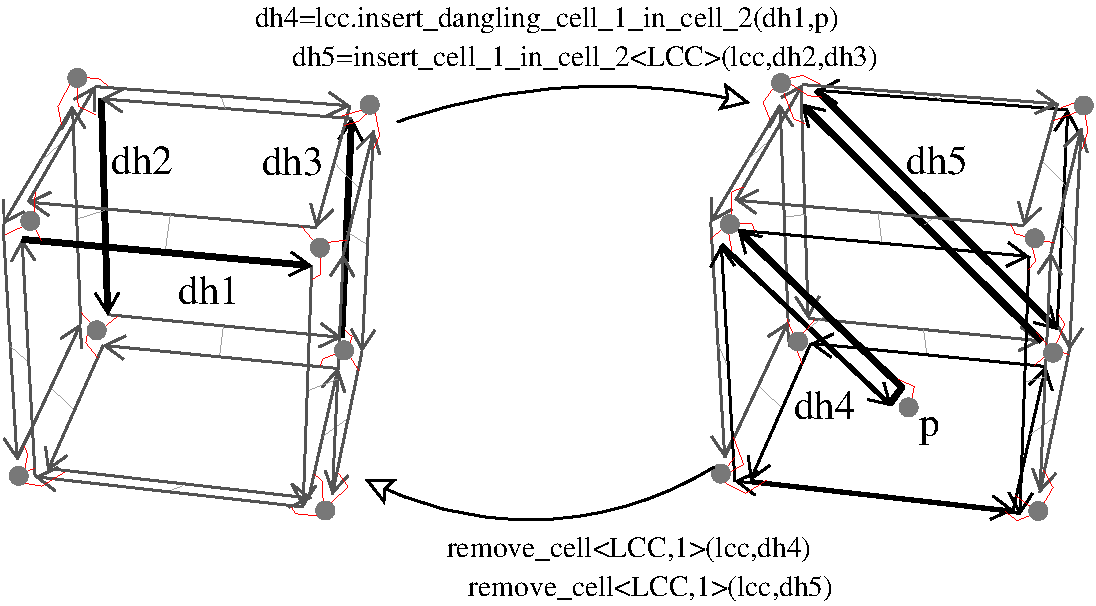
\includegraphics[width=.72\textwidth]{Linear_cell_complex/fig/pdf/insert-edge}
      \end{center}
    \end{ccTexOnly}
    \begin{ccHtmlOnly}
      <CENTER> <A HREF="fig/png/insert-edge.png"><img
      src="fig/png/insert-edge.png" alt=""></A> </CENTER>
    \end{ccHtmlOnly}
    \caption{Example of \ccc{insert_dangling_cell_1_in_cell_2},
      \ccc{insert_cell_1_in_cell_2} and
      \ccc{remove_cell<1>} operations. \textbf{Left}: Initial linear
      cell complex.  \textbf{Right}: After the insertion of a dangling
      1-cell in the 2-cell containing dart \emph{d1}, and of a 1-cell
      in the 2-cell containing dart \emph{d2}. Now if we remove
      the 1-cells containing dart \emph{d4} and \emph{d5},
      we obtain a linear cell complex isomorphic to the initial one.}
    \label{fig-lcc-insert-dangling-edge}
  \end{figure}

  Some examples of use of these operations are given in
  Section~\ref{ssec-5dexample}.

\section{Examples}

\subsection{A 3D Linear Cell Complex}\label{ssec-3D-lcc}

This example uses a 3-dimensional linear cell complex. It creates two
tetrahedra and displays all the points of the linear cell complex
thanks to a \ccc{Vertex_attribute_const_range}. Then, the two
tetrahedra are 3-sewn and we translate all the points of the second
tetrahedron along vector \ccc{v(3,1,1)}.  Since the two tetrahedron
are 3-sewn, this translation moves also the 2-cell of the first
tetrahedron shared with the second one.  This is illustrated by
displaying all the points of each 3-cell. For that we use a
\ccc{std::for_each} and the \ccc{Display_vol_vertices} functor.

\ccIncludeExampleCode{Linear_cell_complex/linear_cell_complex_3.cpp}

The output is:
\begin{verbatim}
Vertices: 1 1 2; 1 0 0; 0 2 0; -1 0 0; 1 1 -3; 1 0 -1; -1 0 -1; 0 2 -1; 
Volume 1 : -1 0 0; 0 2 0; 1 0 0; 1 1 2; 
Volume 2 : 0 2 -1; -1 0 -1; 1 0 -1; 1 1 -3; 
Volume 1 : -1 0 0; 0 2 0; 1 0 0; 1 1 2; 
Volume 2 : 0 2 0; -1 0 0; 1 0 0; 1 1 -3; 
Volume 1 : 2 1 1; 3 3 1; 4 1 1; 1 1 2; 
Volume 2 : 3 3 1; 2 1 1; 4 1 1; 4 2 -2; 
LCC characteristics: #Darts=24, #0-cells=5, #1-cells=9, #2-cells=7, #3-cells=2, #ccs=1, valid=1
\end{verbatim}

The first line gives the points of the linear cell complex before the
\ccc{sew<3>}. There are eight points, four for each tetrahedron.
After the sew, six vertices are merged two by two, thus there are five
vertices. We can see the points of each 3-cell (lines Volume 1 and
Volume 2) before the sew, after the sew and after the translation of
the second volume.  We can see that this translation has also modified
the three common points between the two 3-cells.  The last line shows
the number of cells of the linear cell complex, the number of
connected components, and finally a Boolean to show the validity of
the linear cell complex.

\subsection{A 4D Linear Cell Complex}\label{ssec-5dexample}

This example uses a 4-dimensional linear cell complex embedded in a
5-dimensional ambient space.  It creates two tetrahedra having 5D
points and sews the two tetrahedra by \betaquatre{}. Then we use some high
level operations, displays the number of cells of the linear cell
complex, and checks its validity.  Last we use the reverse operations
to get back to the initial configuration.

\ccIncludeExampleCode{Linear_cell_complex/linear_cell_complex_4.cpp}

The output is:
\begin{verbatim}
#Darts=24, #0-cells=8, #1-cells=12, #2-cells=8, #3-cells=2, #4-cells=2, #ccs=2, valid=1
#Darts=24, #0-cells=4, #1-cells=6, #2-cells=4, #3-cells=1, #4-cells=2, #ccs=1, valid=1
#Darts=28, #0-cells=5, #1-cells=7, #2-cells=4, #3-cells=1, #4-cells=2, #ccs=1, valid=1
#Darts=32, #0-cells=5, #1-cells=8, #2-cells=5, #3-cells=1, #4-cells=2, #ccs=1, valid=1
#Darts=24, #0-cells=8, #1-cells=12, #2-cells=8, #3-cells=2, #4-cells=2, #ccs=2, valid=1
\end{verbatim}

\subsection{A 3D Linear Cell Complex with Colored Vertices}
\label{ssec-exemple-color-vertices}

This example illustrates the way to use a 3D linear cell complex by
adding another information to vertices. For that, we need to define
our own items class.  The difference with the
\ccc{CGAL::Linear_cell_complex_min_items} class is about the definition of
the vertex attribute where we use a \ccc{CGAL::Cell_attribute_with_point}
with a non void info. In this example, the ``vextex color'' is just
given by an \ccc{int} (the second template parameter of the
\ccc{CGAL::Cell_attribute_with_point}).  Lastly, we define the
\ccc{Average_functor} class in order to set the color of a vertex
resulting of the merging of two vertices to the average of the two
initial values. This functor is associated with the vertex attribute
by passing it as template parameter.  Using this items class instead of
the default one is chosen during the instantiation of template
parameters of the \ccc{CGAL::Linear_cell_complex} class.

Now we can use \ccc{LCC_3} in which each vertex is associated with an
attribute containing both a point and an information. In the following
example, we create two cubes, and set the color of the vertices of the
first cube to 1 and of the second cube to 19 (by iterating through two
\ccc{One_dart_per_incident_cell_range<0, 3>} ranges).  Then we
\emph{3-sew} the two cubes along one facet. This operation merges some
vertices (as in the example of Figure~\ref{fig-lcc-exemple-sew}).  We
insert a vertex in the common 2-cell between the two cubes, and set
the information of the new 0-attribute to 5.  In the last loop, we
display the point and the information of each vertex of the linear
cell complex.

\ccIncludeExampleCode{Linear_cell_complex/linear_cell_complex_3_with_colored_vertices.cpp}

The output is:
\begin{verbatim}
point: -1 1 1, color: 10
point: -1 0 1, color: 10
point: -2 0 1, color: 1
point: -2 1 1, color: 1
point: -2 1 0, color: 1
point: -1 1 0, color: 10
point: -1 0 0, color: 10
point: -2 0 0, color: 1
point: 1 1 1, color: 19
point: 1 0 1, color: 19
point: -1 0.5 0.5, color: 5
point: 1 1 0, color: 19
point: 1 0 0, color: 19
\end{verbatim}

Before applying the sew operation, the eight vertices of the first
cube are colored by 1, and the eight vertices of the second cube by
19. After the sew operation, there are eight vertices which are merged
two by two, and due to the average functor, the color of the four
resulting vertices are now 10. Then we insert a vertex in the center
of the common 2-cell between the two cubes.  The coordinates of this
vertex are initialized with the barycenter of the 2-cell
(-1,0.5,0.5), and its color is not initialized by the method, thus we
set its color manually by using the result of
\ccc{insert_barycenter_in_cell<2>} which is a dart incident to the
new vertex.

\section{Design and Implementation History}

This package was developed by Guillaume Damiand, with the help of
Andreas Fabri, S\'ebastien Loriot and Laurent Rineau.  Monique
Teillaud and Bernd G{\"a}rtner contributed to the manual.


% +------------------------------------------------------------------------+
% | Reference manual page: Linear_cell_complex_min_items.tex
% +------------------------------------------------------------------------+
% | 04.02.2010   Guillaume Damiand
% | Package: Linear_cell_complex
% +------------------------------------------------------------------------+
\ccRefPageBegin
%%RefPage: end of header, begin of main body
% +------------------------------------------------------------------------+

\begin{ccRefClass}{Linear_cell_complex_min_items<d>}

\ccInclude{CGAL/Linear_cell_complex_min_items.h}

\ccDefinition
  
The class \ccRefName\ defines the type of darts, which is a
\ccc{Dart_wrapper::Dart<d,LCC>}, and the traits class used.  In
this class, 0-attributes are enabled and associated with
\ccc{Cell_attribute_with_point}.

\ccIsModel
\ccRefConceptPage{LinearCellComplexItems}

\ccParameters
\ccc{d} the dimension of the combinatorial map.

\ccExample

The following example shows one implementation of the
\ccRefName\ class.

\begin{ccExampleCode}
  template <unsigned int d>
  struct Linear_cell_complex_min_items
  {
    template <class LCC>
    struct Dart_wrapper
    {
      typedef CGAL::Dart<d, LCC> Dart;

      typedef CGAL::Cell_attribute_with_point<LCC> Vertex_attrib;    
      typedef CGAL::cpp0x::tuple<Vertex_attrib> Attributes;
    };
  };
\end{ccExampleCode}

\ccSeeAlso
\ccRefIdfierPage{CGAL::Linear_cell_complex<d,d2,LCCTraits,Items,Alloc>}\\
\ccRefIdfierPage{CGAL::Dart<d,CMap>}

\end{ccRefClass}

% +------------------------------------------------------------------------+
%%RefPage: end of main body, begin of footer
\ccRefPageEnd
% EOF
% +------------------------------------------------------------------------+


% +------------------------------------------------------------------------+
% | Reference manual page: Linear_cell_complex_traits.tex
% +------------------------------------------------------------------------+
% | 04.02.2010   Guillaume Damiand
% | Package: Linear_cell_complex
% +------------------------------------------------------------------------+
\ccRefPageBegin
%%RefPage: end of header, begin of main body
% +------------------------------------------------------------------------+

\begin{ccRefClass}{Linear_cell_complex_traits<d,K>}

\ccInclude{CGAL/Linear_cell_complex_traits.h}

\ccDefinition

This geometric traits concept is used in the
\ccc{Linear_cell_complex} class.  It can take as parameter any model of the
concept \ccc{Kernel} (for example any \cgal\ kernel), and defines inner
types and functors corresponding to the given dimension.

\ccIsModel
\ccRefConceptPage{LinearCellComplexTraits}

\ccInheritsFrom
\ccc{K}.

\ccParameters
\ccc{d} the dimension of the kernel,\\
\ccc{K} a model of the concept \ccc{Kernel} if \ccc{d==2} or 
 \ccc{d==3}; a model of the concept \ccc{Kernel_d} otherwise. 

There is a default template arguments for \ccc{K} which is
\ccc{CGAL::Exact_predicates_inexact_constructions_kernel}
if \ccc{d} is 2 or 3, and is \ccc{CGAL::Cartesian_d<double>}
otherwise.

Note that the default argument used for \ccc{K} when
\emph{d}\mygt{}3 does not use exact predicates because operations that
use predicates are only defined in 2D and 3D.

\ccConstants
\ccVariable{static unsigned int ambient_dimension = d;}{}

\ccSeeAlso

\ccRefIdfierPage{CGAL::Linear_cell_complex<d,d2,Traits_,CMItems,Alloc_>}

\end{ccRefClass}
% +------------------------------------------------------------------------+
%%RefPage: end of main body, begin of footer
\ccRefPageEnd
% EOF
% +------------------------------------------------------------------------+

%\input{Linear_cell_complex_ref/Linear_cell_complex_cartesian_traits.tex}
%\input{Linear_cell_complex_ref/Linear_cell_complex_epik_traits.tex}

% +------------------------------------------------------------------------+
% | Reference manual page: Cell_attribute_with_point.tex
% +------------------------------------------------------------------------+
% | 04.02.2010   Guillaume Damiand
% | Package: Linear_cell_complex
% +------------------------------------------------------------------------+
\ccRefPageBegin
%%RefPage: end of header, begin of main body
% +------------------------------------------------------------------------+
\begin{ccRefClass}{Cell_attribute_with_point<LCC,Info_,Tag,OnMerge,OnSplit>}

\ccInclude{CGAL/Cell_attribute_with_point.h}

\ccDefinition
  
The class \ccRefName\ represents an attribute containing a point and
containing an information when \ccc{Info_} is different from void.
This class can typically be used to associate a point to each 0-cell
of a combinatorial map. 

\ccIsModel
\ccRefConceptPage{CellAttributeWithPoint}

\ccInheritsFrom
\ccRefIdfierPage{CGAL::Cell_attribute<CMap,Info_,Tag,OnMerge,OnSplit>}

\ccParameters
\ccc{LCC} must be an instantiation of \ccc{Linear_cell_complex} class,\\
\ccc{Info_} is the type of the information contained in the attribute, \ccc{void} for no information, \\
\ccc{Tag} is \ccc{Tag_true} to enable the storage of a
   \ccc{Dart_handle} of the associated cell, \ccc{Tag_false} otherwise,\\
\ccc{OnMerge} is a functor called when two attributes are merged,  \\
\ccc{OnSplit} is a functor called when one attribute is split in two. 

   By default, \ccc{OnMerge} and \ccc{OnSplit} are equal to
   \ccc{Null_functor}; \ccc{Tag} is equal to
   \ccc{Tag_true}; and \ccc{Info_} is equal to \ccc{void}.

\ccTypes
\ccThree{typedef LCC::Dart_const_handle;}{}{}
\ccTypedef{typedef LCC::Point Point;}{}
\ccGlue
\ccTypedef{typedef LCC::Dart_handle Dart_handle;}{}
\ccGlue
\ccTypedef{typedef LCC::Dart_const_handle Dart_const_handle;}{}

\ccSeeAlso
\ccRefIdfierPage{CGAL::Linear_cell_complex<d,d2,Traits_,CMItems,Alloc_>}\\
\ccRefIdfierPage{CGAL::Linear_cell_complex_min_items<d>}\\
\ccRefIdfierPage{CGAL::Cell_attribute<CMap,Info_,Tag,OnMerge,OnSplit>}

\end{ccRefClass}
% +------------------------------------------------------------------------+
%%RefPage: end of main body, begin of footer
\ccRefPageEnd
% EOF
% +------------------------------------------------------------------------+

%\input{Linear_cell_complex_ref/Cell_attribute_with_point_and_info.tex}


% Third: global functions.
% +------------------------------------------------------------------------+
% | Reference manual page: Linear_cell_complex_constructors.tex
% +------------------------------------------------------------------------+
% | 04.02.2010   Guillaume Damiand
% | Package: Linear_cell_complex
% +------------------------------------------------------------------------+
\ccRefPageBegin
%%RefPage: end of header, begin of main body
% +------------------------------------------------------------------------+

%----------------------------------------------------------------------------
% \begin{ccRefFunction}{make_segment<LCC>}
% \ccInclude{Linear_cell_complex_constructors.h}\\

% \ccFunction{template <class LCC>
%   typename LCC::Dart_handle make_segment(LCC& lcc,
%   const typename LCC::Point& p0,  
%   const typename LCC::Point& p1);}
% {Creates an isolated segment in \ccc{lcc} (two darts linked by \betadeux{}) 
%   having \ccc{p0}, \ccc{p1} as geometry.
%    Returns an handle on the dart associated with \ccc{p0}.
%  \ccPrecond{\ccc{LCC::dimension}\mygeq{}2.}
% }
% %
% \def\LargFig{.3\textwidth}
%   \begin{ccTexOnly}
%     \begin{center}
%       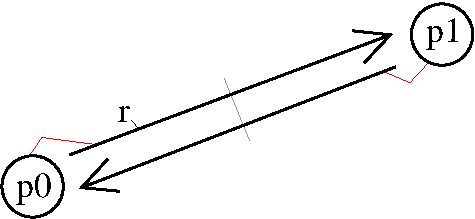
\includegraphics[width=\LargFig]{Linear_cell_complex_ref/fig/pdf/make_segment}
%     \end{center}
%   \end{ccTexOnly}
%   \begin{ccHtmlOnly}
%     <CENTER>
%     <A HREF="fig/png/make_segment.png">
%         <img src="../Linear_cell_complex_ref/fig/png/make_segment.png" alt=""></A>
%     </CENTER>
%     \end{ccHtmlOnly}
%     \centerline{Example of \ccc{r=make_segment(lcc,p0,p1)}.}
% \ccSeeAlso
% \ccRefIdfierPage{CGAL::make_triangle<LCC>}\\
% \ccRefIdfierPage{CGAL::make_quadrangle<LCC>}\\
% \ccRefIdfierPage{CGAL::make_rectangle<LCC>}\\
% %\ccRefIdfierPage{CGAL::make_rectangle2}\\
% %\ccRefIdfierPage{CGAL::make_square}\\
% \ccRefIdfierPage{CGAL::make_tetrahedron<LCC>}\\
% \ccRefIdfierPage{CGAL::make_hexahedron<LCC>}\\
% \ccRefIdfierPage{CGAL::make_iso_cuboid<LCC>}\\
% %\ccRefIdfierPage{CGAL::make_iso_cuboid2}\\
% %\ccRefIdfierPage{CGAL::make_cube}\\
% \end{ccRefFunction}
%----------------------------------------------------------------------------
% \begin{ccRefFunction}{make_triangle<LCC>}
% \ccInclude{Linear_cell_complex_constructors.h}\\

% \ccFunction{template <class LCC>
%   typename LCC::Dart_handle make_triangle(LCC& lcc,
%   const typename LCC::Point& p0,
%   const typename LCC::Point& p1,
%   const typename LCC::Point& p2);}  
% {Creates an isolated triangle in \ccc{lcc} having \ccc{p0}, \ccc{p1}, \ccc{p2} as geometry.
%    Returns an handle on the dart associated with \ccc{p0}.
%  \ccPrecond{\ccc{LCC::dimension}\mygeq{}1.}
% }
% %
% \def\LargFig{.3\textwidth}
%   \begin{ccTexOnly}
%     \begin{center}
%       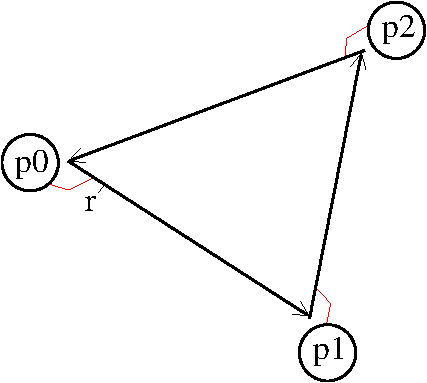
\includegraphics[width=\LargFig]{Linear_cell_complex_ref/fig/pdf/make_triangle}
%     \end{center}
%   \end{ccTexOnly}
%   \begin{ccHtmlOnly}
%     <CENTER>
%     <A HREF="fig/png/make_triangle.png">
%         <img src="../Linear_cell_complex_ref/fig/png/make_triangle.png" alt=""></A>
%     </CENTER>
%     \end{ccHtmlOnly}
%     \centerline{Example of \ccc{r=make_triangle(lcc,p0,p1,p2)}.}
% \ccSeeAlso
% \ccRefIdfierPage{CGAL::make_segment<LCC>}\\
% \ccRefIdfierPage{CGAL::make_quadrangle<LCC>}\\
% \ccRefIdfierPage{CGAL::make_rectangle<LCC>}\\
% %\ccRefIdfierPage{CGAL::make_rectangle2}\\
% %\ccRefIdfierPage{CGAL::make_square}\\
% \ccRefIdfierPage{CGAL::make_tetrahedron<LCC>}\\
% \ccRefIdfierPage{CGAL::make_hexahedron<LCC>}\\
% \ccRefIdfierPage{CGAL::make_iso_cuboid<LCC>}\\
% %\ccRefIdfierPage{CGAL::make_iso_cuboid2}\\
% %\ccRefIdfierPage{CGAL::make_cube}\\
% \end{ccRefFunction}
%----------------------------------------------------------------------------
% \begin{ccRefFunction}{make_quadrangle<LCC>}
% \ccInclude{Linear_cell_complex_constructors.h}\\

% \ccFunction{template <class LCC>
%   typename LCC::Dart_handle make_quadrangle(LCC& lcc,
%   const typename LCC::Point& p0,  
%   const typename LCC::Point& p1,  
%   const typename LCC::Point& p2,  
%   const typename LCC::Point& p3);}  
% {Creates an isolated quadrangle in \ccc{lcc}  having \ccc{p0} ,\ccc{p1}, 
%   \ccc{p2}, \ccc{p3} as geometry.
%    Returns an handle on the dart associated with \ccc{p0}.
%  \ccPrecond{\ccc{LCC::dimension}\mygeq{}1.}
% }
% %
% \def\LargFig{.3\textwidth}
%   \begin{ccTexOnly}
%     \begin{center}
%       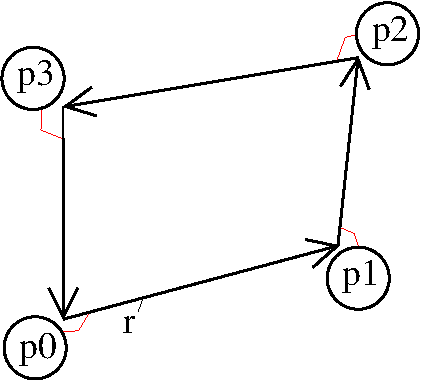
\includegraphics[width=\LargFig]{Linear_cell_complex_ref/fig/pdf/make_quadrilateral}
%     \end{center}
%   \end{ccTexOnly}
%   \begin{ccHtmlOnly}
%     <CENTER>
%     <A HREF="fig/png/make_quadrilateral.png">
%         <img src="../Linear_cell_complex_ref/fig/png/make_quadrilateral.png" alt=""></A>
%     </CENTER>
%     \end{ccHtmlOnly}
%     \centerline{Example of \ccc{r=make_quadrangle(lcc,p0,p1,p2,p3)}.}
% \ccSeeAlso
% \ccRefIdfierPage{CGAL::make_segment<LCC>}\\
% \ccRefIdfierPage{CGAL::make_triangle<LCC>}\\
% \ccRefIdfierPage{CGAL::make_rectangle<LCC>}\\
% %\ccRefIdfierPage{CGAL::make_rectangle2}\\
% %\ccRefIdfierPage{CGAL::make_square}\\
% \ccRefIdfierPage{CGAL::make_tetrahedron<LCC>}\\
% \ccRefIdfierPage{CGAL::make_hexahedron<LCC>}\\
% \ccRefIdfierPage{CGAL::make_iso_cuboid<LCC>}\\
% %\ccRefIdfierPage{CGAL::make_iso_cuboid2}\\
% %\ccRefIdfierPage{CGAL::make_cube}\\
% \end{ccRefFunction}
%----------------------------------------------------------------------------
% \begin{ccRefFunction}{make_rectangle<LCC>}
% \ccInclude{Linear_cell_complex_constructors.h}\\

% \ccFunction{template <class LCC>
%   typename LCC::Dart_handle make_rectangle(LCC& lcc,
%   const typename LCC::Iso_rectangle& ir);}
% {Creates an isolated rectangle in \ccc{lcc} having \ccc{ir} as geometry.
%    Returns an handle on the dart associated with \ccc{ir[0]}.
%  \ccPrecond{\ccc{LCC::dimension}\mygeq{}1 and \ccc{LCC::ambient_dimension}\mygeq{}2.}
% }

% \ccHeading{Requirements}
% \ccc{LCC::Traits} defines \ccc{Iso_rectangle_2} type.

%
% \ccSeeAlso
% \ccRefIdfierPage{CGAL::make_segment}\\
% \ccRefIdfierPage{CGAL::make_triangle}\\
% \ccRefIdfierPage{CGAL::make_quadrangle}\\
% %\ccRefIdfierPage{CGAL::make_square}\\
% \ccRefIdfierPage{CGAL::make_tetrahedron}\\
% \ccRefIdfierPage{CGAL::make_hexahedron}\\
% \ccRefIdfierPage{CGAL::make_iso_cuboid}\\
% \ccRefIdfierPage{CGAL::make_iso_cuboid2}\\
% %\ccRefIdfierPage{CGAL::make_cube}\\
% \end{ccRefFunction}
% %----------------------------------------------------------------------------
% \begin{ccRefFunction}{make_rectangle}
% \ccInclude{Linear_cell_complex_constructors.h}\\

% \ccFunction{template <class LCC>
%   typename LCC::Dart_handle make_rectangle(LCC& lcc,
%   const typename LCC::Point& p0,
%   const typename LCC::Point& p1);}
% {Creates an isolated rectangle in \ccc{lcc} having \ccc{p0} and \ccc{p1} as 
%   diagonal opposite points. Returns an handle on the dart associated with \ccc{p0}.
%  \ccPrecond{\ccc{LCC::dimension}\mygeq{}1 and \ccc{LCC::ambient_dimension}\mygeq{}2.}
% }

% \ccHeading{Requirements}
% \ccc{LCC::Traits} defines \ccc{Iso_rectangle_2} type.

%
% \def\LargFig{.3\textwidth}
%   \begin{ccTexOnly}
%     \begin{center}
%       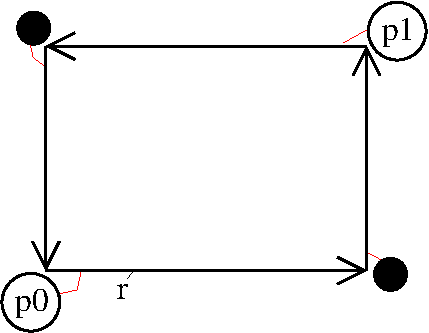
\includegraphics[width=\LargFig]{Linear_cell_complex_ref/fig/pdf/make_rectangle}
%     \end{center}
%   \end{ccTexOnly}
%   \begin{ccHtmlOnly}
%     <CENTER>
%     <A HREF="fig/png/make_rectangle.png">
%         <img src="../Linear_cell_complex_ref/fig/png/make_rectangle.png" alt=""></A>
%     </CENTER>
%     \end{ccHtmlOnly}
%     \centerline{Example of \ccc{r=make_rectangle(lcc,p0,p1)}.}

% \ccSeeAlso
% \ccRefIdfierPage{CGAL::make_segment<LCC>}\\
% \ccRefIdfierPage{CGAL::make_triangle<LCC>}\\
% \ccRefIdfierPage{CGAL::make_quadrangle<LCC>}\\
% %\ccRefIdfierPage{CGAL::make_rectangle2}\\
% %\ccRefIdfierPage{CGAL::make_square}\\
% \ccRefIdfierPage{CGAL::make_tetrahedron<LCC>}\\
% \ccRefIdfierPage{CGAL::make_hexahedron<LCC>}\\
% \ccRefIdfierPage{CGAL::make_iso_cuboid<LCC>}\\
% %\ccRefIdfierPage{CGAL::make_iso_cuboid2}\\
% %\ccRefIdfierPage{CGAL::make_cube}\\
% \end{ccRefFunction}
%----------------------------------------------------------------------------
% \begin{ccRefFunction}{make_square}
% \ccInclude{Linear_cell_complex_constructors.h}\\

% \ccFunction{template <class LCC>
%   typename LCC::Dart_handle make_square(LCC& lcc,
%   const typename LCC::Point& p,
%   typename LCC::FT l);}
% {Creates an isolated square in \ccc{lcc} having \ccc{p}  as based point, and \ccc{l} 
%   as size. Returns an handle on the dart associated with \ccc{p}.
%  \ccPrecond{\ccc{LCC::dimension}$\geq 1$ and \ccc{LCC::ambient_dimension}$\geq 2$.}
% }
% %
% \def\LargFig{.3\textwidth}
%   \begin{ccTexOnly}
%     \begin{center}
%       \includegraphics[width=\LargFig]{Linear_cell_complex_ref/fig/pdf/make_square}
%     \end{center}
%   \end{ccTexOnly}
%   \begin{ccHtmlOnly}
%     <CENTER>
%     <A HREF="fig/png/make_square.png">
%         <img src="../Linear_cell_complex_ref/fig/png/make_square.png" alt=""></A>
%     </CENTER>
%     \end{ccHtmlOnly}
%     \centerline{Example of \ccc{r=make_square(lcc,p,l)}.}
% \ccSeeAlso
% \ccRefIdfierPage{CGAL::make_segment}\\
% \ccRefIdfierPage{CGAL::make_triangle}\\
% \ccRefIdfierPage{CGAL::make_quadrangle}\\
% \ccRefIdfierPage{CGAL::make_rectangle}\\
% \ccRefIdfierPage{CGAL::make_tetrahedron}\\
% \ccRefIdfierPage{CGAL::make_hexahedron}\\
% \ccRefIdfierPage{CGAL::make_iso_cuboid}\\
% %\ccRefIdfierPage{CGAL::make_cube}\\
% \end{ccRefFunction}
%----------------------------------------------------------------------------
% \begin{ccRefFunction}{make_tetrahedron<LCC>}
% \ccInclude{Linear_cell_complex_constructors.h}\\

% \ccFunction{template <class LCC>
%   typename LCC::Dart_handle make_tetrahedron(LCC& lcc,
%   const typename LCC::Point& p0,
%   const typename LCC::Point& p1,
%   const typename LCC::Point& p2,
%   const typename LCC::Point& p3);}
% {Creates an isolated tetrahedron in \ccc{lcc} having \ccc{p0} ,\ccc{p1},\ccc{p2},\ccc{p3} as geometry.
%   Returns an handle on the dart associated with \ccc{p0} and
%   belonging to the 2-cell having \ccc{p0}, \ccc{p1}, \ccc{p2}
%   as coordinates.
%   \ccPrecond{\ccc{LCC::dimension}\mygeq{}2.}
% }
% %
% \def\LargFig{.3\textwidth}
%   \begin{ccTexOnly}
%     \begin{center}
%       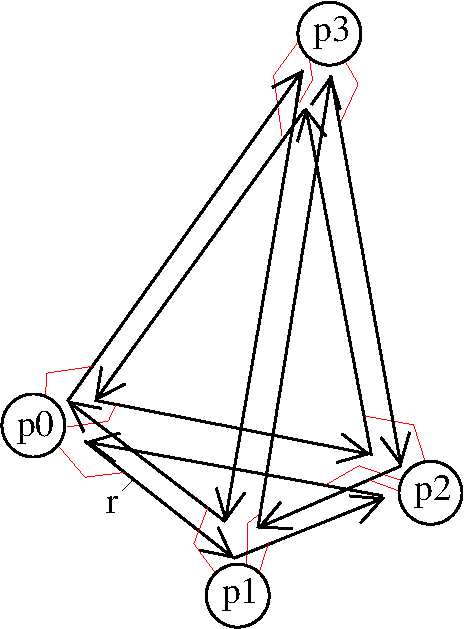
\includegraphics[width=\LargFig]{Linear_cell_complex_ref/fig/pdf/make_tetrahedron}
%     \end{center}
%   \end{ccTexOnly}
%   \begin{ccHtmlOnly}
%     <CENTER>
%     <A HREF="fig/png/make_tetrahedron.png">
%         <img src="../Linear_cell_complex_ref/fig/png/make_tetrahedron.png" alt=""></A>
%     </CENTER>
%     \end{ccHtmlOnly}
%     \centerline{Example of \ccc{r=make_tetrahedron(lcc,p0,p1,p2,p3)}.}
% \ccSeeAlso
% \ccRefIdfierPage{CGAL::make_segment<LCC>}\\
% \ccRefIdfierPage{CGAL::make_triangle<LCC>}\\
% \ccRefIdfierPage{CGAL::make_quadrangle<LCC>}\\
% \ccRefIdfierPage{CGAL::make_rectangle<LCC>}\\
% %\ccRefIdfierPage{CGAL::make_rectangle2}\\
% %\ccRefIdfierPage{CGAL::make_square}\\
% \ccRefIdfierPage{CGAL::make_hexahedron<LCC>}\\
% \ccRefIdfierPage{CGAL::make_iso_cuboid<LCC>}\\
% %\ccRefIdfierPage{CGAL::make_iso_cuboid2}\\
% %\ccRefIdfierPage{CGAL::make_cube}\\
% \end{ccRefFunction}
%----------------------------------------------------------------------------
% \begin{ccRefFunction}{make_hexahedron<LCC>}
% \ccInclude{Linear_cell_complex_constructors.h}\\

% \ccFunction{template <class LCC>
%   typename LCC::Dart_handle make_hexahedron(LCC& lcc,
%   const typename LCC::Point& p0,
%   const typename LCC::Point& p1,
%   const typename LCC::Point& p2,
%   const typename LCC::Point& p3,
%   const typename LCC::Point& p4,
%   const typename LCC::Point& p5,
%   const typename LCC::Point& p6,
%   const typename LCC::Point& p7);}
% {Creates an isolated hexahedron in \ccc{lcc} having \ccc{p0}, \ccc{p1},
% \ccc{p2}, \ccc{p3}, \ccc{p4}, \ccc{p5}, \ccc{p6}, \ccc{p7} as geometry.
%   Returns an handle on the dart associated with \ccc{p0} and
%   belonging to the 2-cell having \ccc{p0}, \ccc{p5}, \ccc{p6}, \ccc{p1}
%   as coordinates.
%   \ccPrecond{\ccc{LCC::dimension}\mygeq{}2.}
% }
% \def\LargFig{.4\textwidth}
%   \begin{ccTexOnly}
%     \begin{center}
%       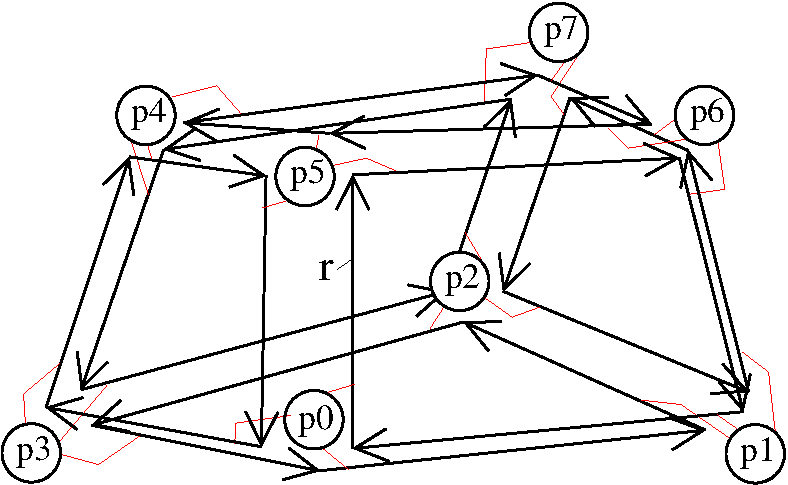
\includegraphics[width=\LargFig]{Linear_cell_complex_ref/fig/pdf/make_hexahedron}
%     \end{center}
%   \end{ccTexOnly}
%   \begin{ccHtmlOnly}
%     <CENTER>
%     <A HREF="fig/png/make_hexahedron.png">
%         <img src="../Linear_cell_complex_ref/fig/png/make_hexahedron.png" alt=""></A>
%     </CENTER>
%     \end{ccHtmlOnly}
%     \centerline{Example of \ccc{r=make_hexahedron(lcc,p0,p1,p2,p3,p4,p5,p6,p7)}.}
% \ccSeeAlso
% \ccRefIdfierPage{CGAL::make_segment<LCC>}\\
% \ccRefIdfierPage{CGAL::make_triangle<LCC>}\\
% \ccRefIdfierPage{CGAL::make_quadrangle<LCC>}\\
% \ccRefIdfierPage{CGAL::make_rectangle<LCC>}\\
% %\ccRefIdfierPage{CGAL::make_rectangle2}\\
% %\ccRefIdfierPage{CGAL::make_square}\\
% \ccRefIdfierPage{CGAL::make_tetrahedron<LCC>}\\
% \ccRefIdfierPage{CGAL::make_iso_cuboid<LCC>}\\
% %\ccRefIdfierPage{CGAL::make_iso_cuboid2}\\
% %\ccRefIdfierPage{CGAL::make_cube}\\
% \end{ccRefFunction}
%----------------------------------------------------------------------------
% \begin{ccRefFunction}{make_iso_cuboid<LCC>}
% \ccInclude{Linear_cell_complex_constructors.h}\\

% \ccFunction{template <class LCC>
%   typename LCC::Dart_handle make_iso_cuboid(LCC& lcc,
%   const typename LCC::Iso_cuboid& ic);}
% {Creates an isolated cuboid in \ccc{lcc} having points in \ccc{ic} as points.
%   Returns an handle on the dart associated with \ccc{ic[0]},
%   and belonging to the 2-cell having
%   \ccc{ic[0]},\ccc{ic[5]}, \ccc{ic[6]},\ccc{ic[1]} as coordinates.
%   \ccPrecond{\ccc{LCC::dimension}\mygeq{}2 and \ccc{LCC::ambient_dimension}\mygeq{}3.}
% }

% \ccHeading{Requirements}
% \ccc{LCC} defines \ccc{Iso_cuboid} type.

%
% \def\LargFig{.4\textwidth}
%   \begin{ccTexOnly}
%     \begin{center}
%       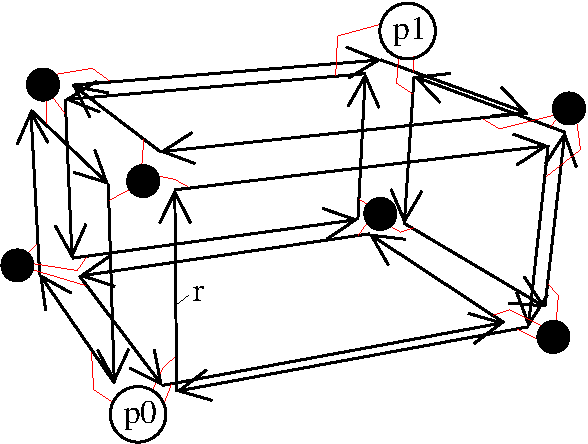
\includegraphics[width=\LargFig]{Linear_cell_complex_ref/fig/pdf/make_cuboid}
%     \end{center}
%   \end{ccTexOnly}
%   \begin{ccHtmlOnly}
%     <CENTER>
%     <A HREF="fig/png/make_cuboid.png">
%         <img src="../Linear_cell_complex_ref/fig/png/make_cuboid.png" alt=""></A>
%     </CENTER>
%     \end{ccHtmlOnly}
%     \centerline{Example of \ccc{r=make_iso_cuboid(lcc,ic)}.}
% \ccSeeAlso
% \ccRefIdfierPage{CGAL::make_segment}\\
% \ccRefIdfierPage{CGAL::make_triangle}\\
% \ccRefIdfierPage{CGAL::make_quadrangle}\\
% \ccRefIdfierPage{CGAL::make_rectangle}\\
% %\ccRefIdfierPage{CGAL::make_rectangle2}\\
% %\ccRefIdfierPage{CGAL::make_square}\\
% \ccRefIdfierPage{CGAL::make_tetrahedron}\\
% \ccRefIdfierPage{CGAL::make_hexahedron}\\
% \ccRefIdfierPage{CGAL::make_iso_cuboid}\\
% %\ccRefIdfierPage{CGAL::make_cube}\\
% \end{ccRefFunction}
% %%----------------------------------------------------------------------------
% \begin{ccRefFunction}{make_iso_cuboid}
% \ccInclude{Linear_cell_complex_constructors.h}\\

% \ccFunction{template <class LCC>
%   typename LCC::Dart_handle make_iso_cuboid(LCC& lcc,
%   const typename LCC::Point& p0,
%   const typename LCC::Point& p1);}
%   {Creates an isolated cuboid in \ccc{lcc} given having \ccc{p0} and
%     \ccc{p1} as diagonal opposite points. We denote by \ccc{ic} the
%     \ccc{Iso_cuboid_3} build from \ccc{p0} and \ccc{p1}.  
%       Returns an handle on the dart associated with \ccc{ic[0]},
%       and belonging to the 2-cell having
%       \ccc{ic[0]},\ccc{ic[5]}, \ccc{ic[6]},\ccc{ic[1]} as coordinates.
%       \ccPrecond{\ccc{LCC::dimension}\mygeq{}2 and \ccc{LCC::ambient_dimension}\mygeq{}3.}
% }

% \ccHeading{Requirements}
% \ccc{LCC} defines \ccc{Iso_cuboid} type.

%
% \def\LargFig{.4\textwidth}
%   \begin{ccTexOnly}
%     \begin{center}
%       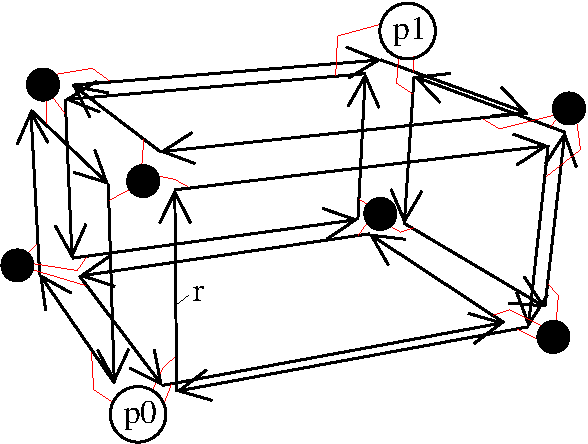
\includegraphics[width=\LargFig]{Linear_cell_complex_ref/fig/pdf/make_cuboid}
%     \end{center}
%   \end{ccTexOnly}
%   \begin{ccHtmlOnly}
%     <CENTER>
%     <A HREF="fig/png/make_cuboid.png">
%         <img src="../Linear_cell_complex_ref/fig/png/make_cuboid.png" alt=""></A>
%     </CENTER>
%     \end{ccHtmlOnly}
%     \centerline{Example of \ccc{r=make_iso_cuboid(lcc,p0,p1)}.}

% \ccSeeAlso
% \ccRefIdfierPage{CGAL::make_segment<LCC>}\\
% \ccRefIdfierPage{CGAL::make_triangle<LCC>}\\
% \ccRefIdfierPage{CGAL::make_quadrangle<LCC>}\\
% \ccRefIdfierPage{CGAL::make_rectangle<LCC>}\\
% %\ccRefIdfierPage{CGAL::make_rectangle2}\\
% %\ccRefIdfierPage{CGAL::make_square}\\
% \ccRefIdfierPage{CGAL::make_tetrahedron<LCC>}\\
% \ccRefIdfierPage{CGAL::make_hexahedron<LCC>}\\
% %\ccRefIdfierPage{CGAL::make_iso_cuboid2}\\
% %\ccRefIdfierPage{CGAL::make_cube}\\
% \end{ccRefFunction}
%----------------------------------------------------------------------------
% \begin{ccRefFunction}{make_cube}
% \ccInclude{Linear_cell_complex_constructors.h}\\

% \ccFunction{typename LCC::Dart_handle make_cube(LCC& lcc,
%                                     const typename LCC::Point& p,
%                                     typename LCC::FT l);}
% {Creates an isolated cube in \ccc{lcc} having \ccc{p} as based point, and
%   \ccc{l} as size.
%   Returns an handle on the dart associated with \ccc{p},
%   and belonging to the 2-cell having
%   \ccc{p},\ccc{p}+(0,0,\ccc{l}), \ccc{p}+(\ccc{l},0,\ccc{l}), \ccc{a}+(\ccc{l},0,0). 
%   as coordinates.
%   \ccPrecond{\ccc{LCC::dimension}$\geq 2$ and \ccc{LCC::ambient_dimension}$\geq 3$.}
% }
% %
% \def\LargFig{.3\textwidth}
%   \begin{ccTexOnly}
%     \begin{center}
%       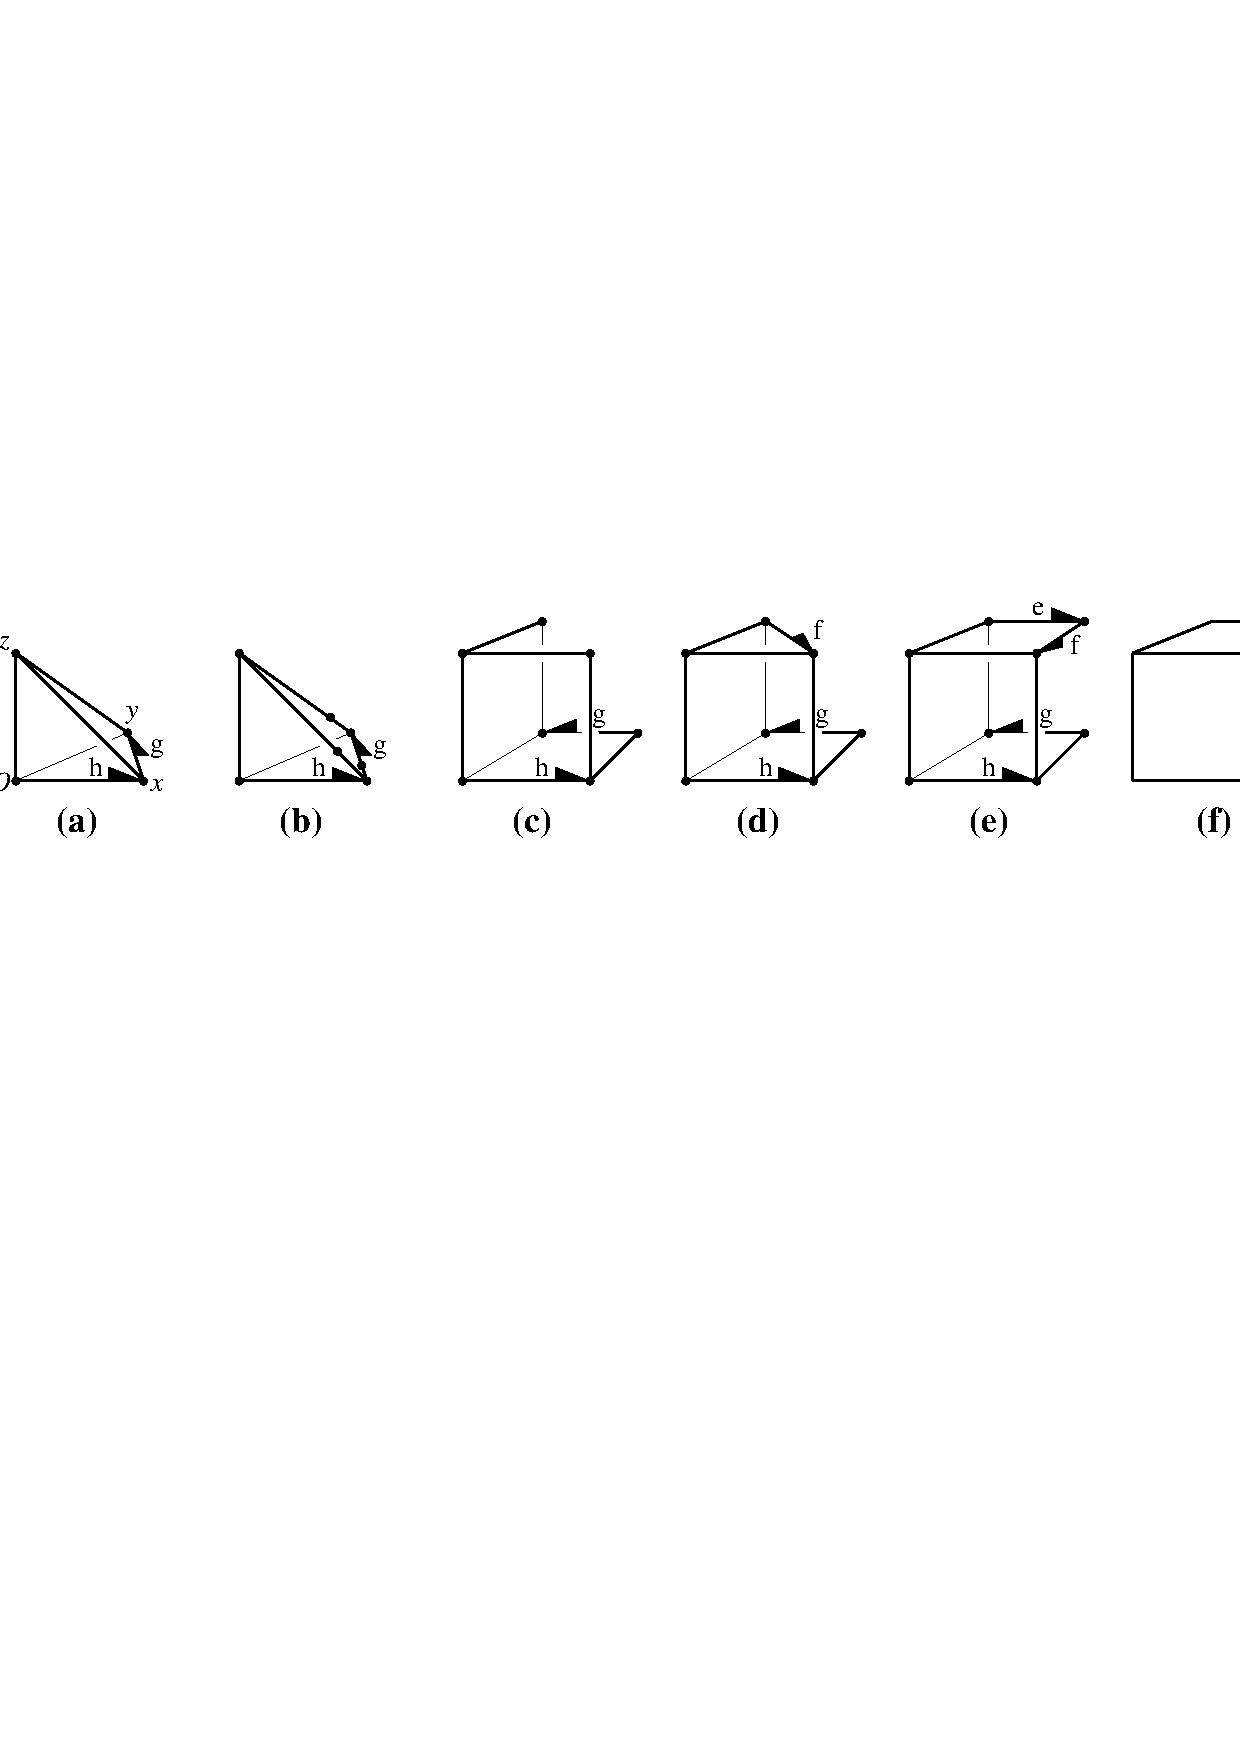
\includegraphics[width=\LargFig]{Linear_cell_complex_ref/fig/pdf/make_cube}
%     \end{center}
%   \end{ccTexOnly}
%   \begin{ccHtmlOnly}
%     <CENTER>
%     <A HREF="fig/png/make_cube.png">
%         <img src="../Linear_cell_complex_ref/fig/png/make_cube.png" alt=""></A>
%     </CENTER>
%     \end{ccHtmlOnly}
%     \centerline{Example of \ccc{r=make_cube(lcc,p,l)}.}
% \ccSeeAlso
% \ccRefIdfierPage{CGAL::make_segment}\\
% \ccRefIdfierPage{CGAL::make_triangle}\\
% \ccRefIdfierPage{CGAL::make_quadrangle}\\
% \ccRefIdfierPage{CGAL::make_rectangle}\\
% %\ccRefIdfierPage{CGAL::make_square}\\
% \ccRefIdfierPage{CGAL::make_tetrahedron}\\
% \ccRefIdfierPage{CGAL::make_hexahedron}\\
% \ccRefIdfierPage{CGAL::make_iso_cuboid}\\
% \end{ccRefFunction}
%----------------------------------------------------------------------------
\begin{ccRefFunction}{import_from_plane_graph<LCC>}
\ccInclude{Linear_cell_complex_constructors.h}\\

\ccFunction{template<class LCC>
  typename LCC::Dart_handle import_from_plane_graph(LCC& lcc,
  std::istream& ais);}
{Imports an embedded plane graph read from \ccc{ais} into \ccc{lcc}. 
  Objects are added in \ccc{lcc}, existing darts are not modified.
  Returns a dart created during the import.
  \ccPrecond{\ccc{LCC::dimension}\mygeq{}2 and \ccc{LCC::ambient_dimension}==2.}
}

\ccHeading{File format} The file format must be the following.  First
the number of vertices and the number of edges of the planar graph.
Then, for each vertex of the planar graph, the coordinates of the
\myith{} vertex (two numbers for $x$ and $y$ coordinates). The first
vertex index is 0. Then for each edge of the planar graph, the two
indices of the two vertices (two numbers between 0 and the number of
vertices minus 1).

% \begin{itemize}
% \item first line: \verb|nbvertices nbedges|;
% \item \verb|nbvertices| lines: \verb|x y| 
% \item \verb|nbedges| lines: \verb|i j| the index of the two vertices of the edge (first vertex
% being 0).
% \end{itemize}

Here a small example:
\begin{verbatim}
5 6
1.0 3.0   0.0 2.0   2.0 2.0   0.0 0.0   2.0 0.0
0 1   0 2   1 2   1 3   2 4   3 4
\end{verbatim}
%
\def\LargFig{.5\textwidth}
  \begin{ccTexOnly}
    \begin{center}
      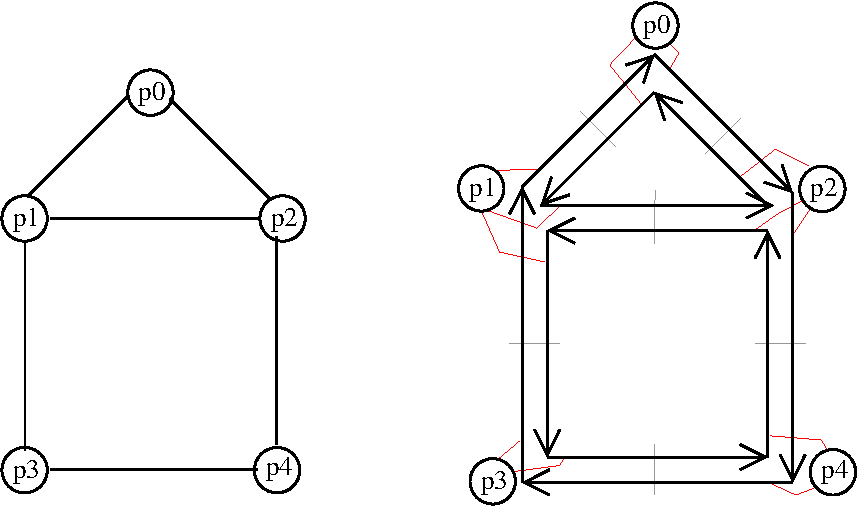
\includegraphics[width=\LargFig]{Linear_cell_complex_ref/fig/pdf/import_graph}
    \end{center}
  \end{ccTexOnly}
  \begin{ccHtmlOnly}
    <CENTER>
    <A HREF="fig/png/import_graph.png">
        <img src="../Linear_cell_complex_ref/fig/png/import_graph.png" alt=""></A>
    </CENTER>
    \end{ccHtmlOnly}
    \begin{center}
      Example of \ccc{import_graph} reading the above file as istream. \\
      \textbf{Left}: A planar graph embedded in the plane with 
      \emph{P0}=(1.0,3.0), \emph{P1}=(0.0,2.0), \emph{P2}=(2.0,2.0), \emph{P3}=(0.0,0.0), \emph{P4}=(2.0,0.0).
      \textbf{Right}: the 2D linear cell complex reconstructed.
      \end{center}
\ccSeeAlso
\ccRefIdfierPage{CGAL::import_from_triangulation_3<LCC,Triangulation>}\\
\ccRefIdfierPage{CGAL::import_from_polyhedron<LCC,Polyhedron>}\\
\end{ccRefFunction}
%----------------------------------------------------------------------------
\begin{ccRefFunction}{import_from_triangulation_3<LCC,Triangulation>}
\ccInclude{Linear_cell_complex_constructors.h}\\

\ccFunction{template <class LCC,class Triangulation_>
   typename LCC::Dart_handle import_from_triangulation_3(LCC& lcc,
   const Triangulation_ &atr);}
 {Imports \ccc{atr} (a \ccc{Triangulation_3}) into \ccc{lcc}. 
   Objects are added in \ccc{lcc}, existing darts are not modified.
   Returns a dart created during the import.
   \ccPrecond{\ccc{LCC::dimension}\mygeq{}3.}
 }
\ccSeeAlso
\ccRefIdfierPage{CGAL::import_from_plane_graph<LCC>}\\
\ccRefIdfierPage{CGAL::import_from_polyhedron<LCC,Polyhedron>}\\
\end{ccRefFunction}
%----------------------------------------------------------------------------
\begin{ccRefFunction}{import_from_polyhedron<LCC,Polyhedron>}
\ccInclude{Linear_cell_complex_constructors.h}\\

\ccFunction{template<class LCC,class Polyhedron>
  typename LCC::Dart_handle import_from_polyhedron(LCC& lcc, 
                                       Polyhedron &apoly);}
{Imports \ccc{apoly} (a \ccc{Polyhedron}) into \ccc{lcc}. Objects are added in \ccc{lcc},
  existing darts are not modified.
  Returns a dart created during the import. 
  \ccPrecond{\ccc{LCC::dimension}\mygeq{}2.}
}
\ccSeeAlso
\ccRefIdfierPage{CGAL::import_from_plane_graph<LCC>}\\
\ccRefIdfierPage{CGAL::import_from_triangulation_3<LCC,Triangulation>}\\
\end{ccRefFunction}
% +------------------------------------------------------------------------+
%%RefPage: end of main body, begin of footer
\ccRefPageEnd
% EOF
% +------------------------------------------------------------------------+
    
% +------------------------------------------------------------------------+
% | Reference manual page: Linear_cell_complex_operations.tex
% +------------------------------------------------------------------------+
% | 04.02.2010   Guillaume Damiand
% | Package: Combinatorial_map
% +------------------------------------------------------------------------+
\ccRefPageBegin
%%RefPage: end of header, begin of main body
% +------------------------------------------------------------------------+

% \begin{ccRefFunction}{barycenter<LCC,i>}
% \ccInclude{Linear_cell_complex_operations.h}\\
% \ccFunction{template<class LCC, unsigned int i>
%   typename LCC::Point barycenter(const LCC& lcc, 
%   typename LCC::Dart_const_handle dh);}
% {Returns the barycenter of the \emph{i}-cell containing \ccc{dh}.
%   \ccPrecond{0\myleq{}\emph{i}\myleq{}\ccc{LCC::dimension} and \ccc{*dh}\myin{}\ccc{lcc.darts()}.}
% }

%   for example $i=2$ for facet, or $i=3$ for volume).\\
% \ccCommentHeading{Template parameter}\\
% \ccc{LCC} must be a model of the \ccc{CombinatorialLCCWithPoints} concept.
% \ccCommentHeading{Parameters} \\
% \ccc{lcc}: the combinatorial map used;\\
% \ccc{adart}: a dart belonging to the cell;\\
% \ccCommentHeading{Returns} \\
%    the barycenter of the cell.
% }
% \ccSeeAlso
% \ccRefIdfierPage{CGAL::compute_normal_of_cell_0<LCC>}\\
% \ccRefIdfierPage{CGAL::compute_normal_of_cell_2<LCC>}\\
% \ccRefIdfierPage{CGAL::insert_center_cell_0_in_cell_2<LCC>}\\
% \end{ccRefFunction}
%--------------------------------------------------------------------------------
\begin{ccRefFunction}{compute_normal_of_cell_0<LCC>}
\ccInclude{Linear_cell_complex_operations.h}\\
\ccFunction{template <class LCC>
typename LCC::Vector compute_normal_of_cell_0(const LCC& lcc, 
typename LCC::Dart_const_handle dh);}
{Returns the normal vector of the 0-cell containing \ccc{dh}; i.e. the average of
  all the normal vectors of the 2-cells incident to the 0-cell containing \ccc{dh}.
  \ccPrecond{\ccc{LCC::ambient_dimension}==3 and \ccc{*dh}\myin{}\ccc{lcc.darts()}.}
}

\ccSeeAlso
%\ccRefIdfierPage{CGAL::barycenter<LCC,i>}\\
\ccRefIdfierPage{CGAL::compute_normal_of_cell_2<LCC>}\\
\end{ccRefFunction}
%--------------------------------------------------------------------------------
\begin{ccRefFunction}{compute_normal_of_cell_2<LCC>}
\ccInclude{Linear_cell_complex_operations.h}\\
\ccFunction{template <class LCC>
typename LCC::Vector compute_normal_of_cell_2(const LCC& lcc, 
typename LCC::Dart_const_handle dh);}
{Returns the normal vector of the 2-cell containing \ccc{dh}.
  \ccPrecond{\ccc{LCC::ambient_dimension}==3 and \ccc{*dh}\myin{}\ccc{lcc.darts()}.}
}

\ccSeeAlso
%\ccRefIdfierPage{CGAL::barycenter<LCC,i>}\\
\ccRefIdfierPage{CGAL::compute_normal_of_cell_0<LCC>}\\
\end{ccRefFunction}
%--------------------------------------------------------------------------------
% \begin{ccRefFunction}{insert_barycenter_in_cell<LCC,i>}
% \ccInclude{Combinatorial_map_operations.h}\\

% \ccFunction{template <class LCC, unsigned int i>
%   typename LCC::Dart_handle insert_barycenter_in_cell(LCC& lcc,
%                                         typename LCC::Dart_handle dh);}
% {Inserts a point in the barycenter of the \emph{i}-cell containing \ccc{dh}.
%   Returns an handle on one dart of this cell.  
%   \ccPrecond{\ccc{LCC::dimension}\mygeq{}1 and \ccc{*dh}\myin{}\ccc{lcc.darts()}.}\\
% %  \begin{ccAdvanced}
%     If \emph{i}-attributes are non void, 
%     \ccc{Attribute_type<i>::type::On_split}(\emph{a},\emph{a'}) is called,
%     with \emph{a} the original \emph{i}-attribute associated
%     with \emph{dh} and \emph{a'} each new \emph{i}-attribute created during the operation.
% %  \end{ccAdvanced}
% }

% \ccSeeAlso
% \ccRefIdfierPage{CGAL::insert_cell_0_in_cell_1<LCC>}\\
% \ccRefIdfierPage{CGAL::insert_cell_0_in_cell_2<LCC>}\\
% \ccRefIdfierPage{CGAL::insert_barycenter_in_cell<LCC,i>}\\
% \ccRefIdfierPage{CGAL::insert_dangling_cell_1_in_cell_2<LCC>}\\
% \end{ccRefFunction}
%--------------------------------------------------------------------------------
% \begin{ccRefFunction}{insert_point_in_cell<LCC,i>}
% \ccInclude{Combinatorial_map_operations.h}\\

% \ccFunction{template <class LCC, unsigned int i>
%   typename LCC::Dart_handle insert_point_in_cell(LCC& lcc,
%                                         typename LCC::Dart_handle dh,
%                                         typename LCC::Point p);}
% {Inserts a point, copy of \ccc{p}, in the \emph{i}-cell containing \ccc{dh}.
%   Returns an handle on one dart of this cell.  
%   \ccPrecond{\ccc{LCC::dimension}\mygeq{}1 and \ccc{*dh}\myin{}\ccc{lcc.darts()}.}\\
% %  \begin{ccAdvanced}
%     If \emph{i}-attributes are non void, 
%     \ccc{Attribute_type<i>::type::On_split}(\emph{a},\emph{a'}) is called, 
%     with $a$ the original \emph{i}-attribute associated
%     with $dh$ and $a'$ each new \emph{i}-attribute created during the operation.
% %  \end{ccAdvanced}
% }

% \ccSeeAlso
% \ccRefIdfierPage{CGAL::insert_barycenter_in_cell<LCC,i>}\\
% \ccRefIdfierPage{CGAL::insert_dangling_cell_1_in_cell_2<LCC>}\\
% \end{ccRefFunction}
%--------------------------------------------------------------------------------
% \begin{ccRefFunction}{insert_cell_0_in_cell_2<LCC>}
% \ccInclude{Linear_cell_complex_operations.h}\\
% \ccFunction{template <class LCC>
%       typename LCC::Dart_handle insert_cell_0_in_cell_2(LCC & lcc,
%       typename LCC::Dart_handle dh,
%       typename LCC::Point p);}
% {Inserts a 0-cell in the 2-cell containing \ccc{dh}, associated with
%   a 0-attribute having \ccc{p} as point.
% The 2-cell is splitted in triangles, one for each initial edge of the facet.
% Returns an handle on one dart belonging to the new 0-cell.
% \ccPrecond{\ccc{LCC::dimension}\mygeq{}2 and \ccc{*dh}\myin{}\ccc{lcc.darts()}.}\\
% %  \begin{ccAdvanced}
%     If 2-attributes are non void, 
%     \ccc{Attribute_type<2>::type::On_split}(\emph{a},\emph{a'}) is called, 
%     with \emph{a} the original 2-attribute associated
%     with \emph{dh} and \emph{a'} each new 2-attribute created during the operation.
% %  \end{ccAdvanced}
% }

% \ccSeeAlso
% \ccRefIdfierPage{CGAL::insert_middle_cell_0_in_cell_1<LCC>}\\
% \ccRefIdfierPage{CGAL::insert_cell_0_in_cell_1<LCC>}\\
% \ccRefIdfierPage{CGAL::insert_center_cell_0_in_cell_2<LCC>}\\
% \ccRefIdfierPage{CGAL::insert_dangling_cell_1_in_cell_2<LCC>}\\
% \end{ccRefFunction}
%--------------------------------------------------------------------------------
% \begin{ccRefFunction}{insert_center_cell_0_in_cell_2<LCC>}
% \ccInclude{Linear_cell_complex_operations.h}\\
% \ccFunction{template <class LCC>
%       typename LCC::Dart_handle insert_center_cell_0_in_cell_2(LCC & lcc,
%       typename LCC::Dart_handle dh);}
% {Inserts a 0-cell in the barycenter of the 2-cell containing \ccc{dh}.
% The 2-cell is splitted in triangles, one for each initial edge of the facet.
% Returns an handle on one dart belonging to the new 0-cell.
% \ccPrecond{\ccc{LCC::dimension}\mygeq{}2 and \ccc{*dh}\myin{}\ccc{lcc.darts()}.}\\
% %  \begin{ccAdvanced}
%     If 2-attributes are non void,
%     \ccc{Attribute_type<2>::type::On_split}(\emph{a},\emph{a'}) is called, 
%     with \emph{a} the original 2-attribute associated
%     with \emph{dh} and \emph{a'} each new 2-attribute created during the operation.
% %  \end{ccAdvanced}
% }

% \ccSeeAlso
% \ccRefIdfierPage{CGAL::barycenter<LCC,i>}\\
% \ccRefIdfierPage{CGAL::insert_middle_cell_0_in_cell_1<LCC>}\\
% \ccRefIdfierPage{CGAL::insert_cell_0_in_cell_1<LCC>}\\
% \ccRefIdfierPage{CGAL::insert_cell_0_in_cell_2<LCC>}\\
% \ccRefIdfierPage{CGAL::insert_dangling_cell_1_in_cell_2<LCC>}\\
% \end{ccRefFunction}
%--------------------------------------------------------------------------------
% \begin{ccRefFunction}{insert_dangling_cell_1_in_cell_2<LCC>}
% \ccInclude{Combinatorial_map_operations.h}\\

% \ccFunction{template <class LCC>
%   typename LCC::Dart_handle insert_dangling_cell_1_in_cell_2(LCC& lcc,
%                                          typename LCC::Dart_handle dh,
%                                          typename LCC::Point p);}
% {Inserts a 1-cell in a the 2-cell containing \ccc{adart}, the 1-cell
%   being attached only by one of its vertex to the 0-cell containing \ccc{dh}.
%   The second vertex is associated with a new 0-attribute containing a copy of
%   \ccc{p} as point. Returns an handle on one dart belonging to the new 0-cell.
%   \ccPrecond{\ccc{LCC::dimension}\mygeq{}2 and \ccc{*dh}\myin{}\ccc{lcc.darts()}.}
% }
% \ccSeeAlso
% \ccRefIdfierPage{CGAL::insert_middle_cell_0_in_cell_1<LCC>}\\
% \ccRefIdfierPage{CGAL::insert_cell_0_in_cell_1<LCC>}\\
% \ccRefIdfierPage{CGAL::insert_cell_0_in_cell_2<LCC>}\\
% \ccRefIdfierPage{CGAL::insert_center_cell_0_in_cell_2<LCC>}\\
% \end{ccRefFunction}
%--------------------------------------------------------------------------------

% +------------------------------------------------------------------------+
%%RefPage: end of main body, begin of footer
\ccRefPageEnd
% EOF
% +------------------------------------------------------------------------+


%% EOF
